%\chapter{Normal Modes}
\chapter{简正模式}

%%%
%%%
均匀转动参照系中地球性质的时不变性,使得我们很自然地寻求在时间上为谐波函数的解:
%%%
\eq
\label{4.eq1}
\bs(\bx,t)=\bs(\bx)\exp(i\omega t).
\en
%%%
%%%
我们称~$\omega$~为地球的角{\em 本征频率},称位移场~$\bs(\bx)$~为相应的{\em 本征函数}。在本章中我们来探究这些简正模式解的本质。
%%%

%%%
%%%
寻找形如~(\ref{4.eq1})~式的振荡解等价于利用如下关系将运动方程和边界条件转换到频率域:
%%%
\eq
\label{4.FTdef}
\bs(\bx,\omega)=\int_{-\infty}^{\infty}\bs(\bx,t)\exp(-i\omega t)\,dt.
\en
%%%
%%%
无论哪种做法,我们都是通过~$\p_t\longleftrightarrow i\omega$~这一替换从一个域转到另一个域。(\ref{4.FTdef})~式的傅里叶变换定义是最适合于考虑地球自由振荡的;值得注意的是,这里指数上的符号约定与行波分析中所采用的习惯~(Aki \& Richards \citeyear{aki&richards80}) 不同。
%%%

%%%
%%%
本章的大部分工作是将第3章的时间域结果简单地转换到频率域。对大多数变量,我们在时间域和频率域使用相同的符号;这应该不会导致任何混淆。由于多种原因,将无自转地球与有自转地球这两种情况分开考虑会更为方便。我们先考虑较简单的无自转~($\bOmega=\bzero$)~情况,再将更为复杂但相对应的具有自转弹性地球模型的讨论放到一个单独的带星号小节。
%%%

%\section{Non-Rotating Earth Model}
\section{无自转地球模型}
\index{normal mode!non-rotating Earth|(}%
\label{4.sec.nonrot}

%%%
%%%
若要得到自转地球的本征频率~$\omega$~与本征函数~$\bs$,我们求解方程:
%%%
\eq
\label{4.nrmodeqn}
-\omega^2\rho^0\bs-\bdel\cdot\bT^{\rm PK1}+\rho^0\bdel\phi^{\rm E1}
+\rho^0\bs\cdot\bdel\bdel\phi^0=\bzero\quad\mbox{在 $\earth$ 内},
\en
%%%
%%%
以及边界条件
%%%
\eq
\label{4.bc1}
\bnh\cdot\bT^{\rm PK1}=\bzero\quad\mbox{在 $\p\earth$ 上},
\en
\eq
\label{4.bc2}
[\bnh\cdot\bT^{\rm PK1}]^+_-=\bzero\quad\mbox{在 $\Sigma_{\rm SS}$ 上},
\en
\eq
\label{4.bc4}
[\bt^{\rm PK1}]^+_-
=\bnh[\bnh\cdot\bt^{\rm PK1}]^+_-
=\bzero\quad\mbox{在 $\Sigma_{\rm FS}$ 上}.
\en
%%%
不失一般性,我们可认为无自转地球模型的本征频率平方~$\omega^2$~和本征函数~$\bs$~皆为{\em 实的\/}:
%%%
\eq
(\omega^2)^*=\omega^2,\qquad\bs^*=\bs,
\en
%%%
其中星号表示复共轭。转换后的动量方程~(\ref{4.nrmodeqn})~对~$\omega^2$~的依赖性表明,对于每个实的本征函数~$\bs$~有两个相关的本征频率;如果~$\omega^2 > 0$,本征频率为实数 $\pm\omega$,而如果~$\omega^2 < 0$,则它们为虚数 $\pm i|\omega|$。为简单起见,此后我们将假定所有的本征频率都是实数;在~\ref{4.sec.stable}~节中,我们将推导出一个确保该假定成立的动力学稳定性条件。
%%%

%\subsection{Hermitian operator formulation}
\subsection{厄米特算子方法}
\index{Hermitian operator|(}%
\index{operator!Hermitian|(}%
\index{operator!self-adjoint|(}%
\index{self-adjoint operator|(}%
\label{4.sec.nrHerm}

%%%
为了简明起见,我们将本征解~$\pm\omega$~和~$\bs$~满足的方程~(\ref{4.nrmodeqn})--(\ref{4.bc4})~改写为符号化形式
%%%
\eq
\label{4.Vswsqs}
\sH\bs=\omega^2\bs,
\en
以及在~$\Sigma=\p\earth\cup\Sigma_{\rm SS}\cup\Sigma_{\rm FS}$~上的边界条件~(\ref{4.bc1})--(\ref{4.bc4})。
这里的符号~$\sH$~表示在地球模型~$\earth$~内的{\em 积分-微分算子\/}
%%%
\index{integro-differential operator}%
\index{operator!integro-differential}%
\eq
\label{4.Vopdef}
\rho^0\sH\bs=-\bdel\cdot\bT^{\rm PK1}+\rho^0\bdel\phi^{\rm E1}
+\rho^0\bs\cdot\bdel\bdel\phi^0
\en
$\omega^2$~和~$\bs$~可以被视为线性算子~$\sH$~的本征值和相应的本征函数。我们目前暂且视欧拉势函数微扰~$\phi^{\rm E1}$~为~$\bs$~的已知泛函,由~(\ref{3.phiE1int2})~给定。
%%%

我们定义~$\earth$~内部任意两个分段光滑实函数~$\bs$~和~$\bs'$~的内积~$\langle\bs,\bs'\rangle$~为 
%%%
\eq
\label{4.inprod}
\langle\bs,\bs'\rangle=\int_{\subearth}\rho^0\bs\cdot\bs'\,dV.
\en
对于这样的内积定义,算子~$\sH$~是{\em 厄米特\/}或{\em 自共轭\/}算子,即
%%%
\eq
\label{4.HERM}
\langle\bs,\sH\bs'\rangle=\langle\sH\bs,\bs'\rangle
=\langle\bs',\sH\bs\rangle.
\en
%%%
(\ref{4.HERM})~式很容易被验证,其左右两侧可以显式分别表示为
%%%
\eq
\langle\bs,\sH\bs'\rangle=\int_{\subearth}\bs\cdot
[-\bdel\cdot\bT^{{\rm PK1}\prime}+\rho^0\bdel\phi^{{\rm E1}\prime}
+\rho^0\bs'\cdot\bdel\bdel\phi^0]\,dV,
\en
\eq
\langle\bs',\sH\bs\rangle=\int_{\subearth}\bs'\cdot
[-\bdel\cdot\bT^{\rm PK1}+\rho^0\bdel\phi^{\rm E1}
+\rho^0\bs\cdot\bdel\bdel\phi^0]\,dV,
\en
其中~$\bT^{{\rm PK1}\prime}$~和~$\phi^{{\rm E1}\prime}$~分别为与带撇号的位移~$\bs'$~相关的~Piola-Kirchhoff~应力增量和欧拉势函数微扰。应用高斯定理,以及在~$\p\earth$~和~$\Sigma_{\rm SS}$~上的边界条件~(\ref{4.bc1})~和~(\ref{4.bc2}),我们得到
%%%
\eqa
\label{4.ssprint}
\lefteqn{
\langle\bs,\sH\bs'\rangle=\int_{\subearth}
[\bdel\bs\!:\!\bLambda\!:\!\bdel\bs'+\rho^0\bs\cdot\bdel\phi^{{\rm E1}\prime}
+\rho^0\bs\cdot\bdel\bdel\phi^0\cdot\bs']\,dV} \nonumber \\
&&\mbox{}\qquad\qquad+\int_{\Sigma_{\rm FS}}[\bnh\cdot
\bT^{{\rm PK1}\prime}\cdot\bs]^+_-\,d\Sigma,
\ena
\eqa
\label{4.ssprint2}
\lefteqn{
\langle\bs',\sH\bs\rangle=\int_{\subearth}
[\bdel\bs'\!:\!\bLambda\!:\!\bdel\bs+\rho^0\bs'\cdot\bdel\phi^{\rm E1}
+\rho^0\bs'\cdot\bdel\bdel\phi^0\cdot\bs]\,dV} \nonumber \\
&&\mbox{}\qquad\qquad+\int_{\Sigma_{\rm FS}}[\bnh\cdot
\bT^{\rm PK1}\cdot\bs']^+_-\,d\Sigma.
\ena
由于Maxwell关系~$\Lambda_{ijkl}=\Lambda_{klij}$~和引力等式
%%%
\eqa
\label{4.gravid}
\lefteqn{
\int_{\subearth}\rho^0\bs\cdot\bdel\phi^{{\rm E1}\prime}\,dV
=\int_{\subearth}\rho^0\bs'\cdot\bdel\phi^{\rm E1}\,dV} \nonumber \\
&&\mbox{}=-\int_{\subearth}\int_{\subearth}(\rho^0\bs
\cdot\bPi\cdot\rho^{0\prime}\bs')\,dV\,dV',
\ena
(\ref{4.ssprint})~和~(\ref{4.ssprint2})~两式右边的体积分是相等的,而上式中对称的积分核~$\bPi(\bx,\bx')=\bPi^{\rm T}(\bx',\bx)$~由~(\ref{3.bPidef})~式给定。在~$\Sigma_{\rm FS}$~上的面积分也是相等的,因此从~(\ref{3.jump})~和~(\ref{3.jump2})~我们得到
%%%
\eqa
\lefteqn{\int_{\Sigma_{\rm FS}}[\bnh\cdot
\bT^{{\rm PK1}\prime}\cdot\bs]^+_-\,d\/\Sigma
=\int_{\Sigma_{\rm FS}}[\bnh\cdot
\bT^{\rm PK1}\cdot\bs']^+_-\,d\/\Sigma} \nonumber \\
& & \mbox{}=\half\int_{\Sigma_{\rm FS}}[\varpi^0\bs\cdot(\bdel^{\Sigma}\bs')\cdot\bnh
+\varpi^0\bs'\cdot(\bdel^{\Sigma}\bs)\cdot\bnh \\
& & \mbox{}\qquad\qquad-(\bnh\cdot\bs)\bdel^{\Sigma}\cdot(\varpi^0\bs')
-(\bnh\cdot\bs')\bdel^{\Sigma}\cdot(\varpi^0\bs)]^+_-\,d\/\Sigma. \nonumber 
\ena
%%%
值得注意的是,在建立弹性-引力算子~$\sH$~的厄米特性质中所需要的处理细节与第~3.8~节中建立能量守恒定律~$d\/\sE\hspace{-0.3 mm}/\hspace{-0.3 mm}dt=0$~所做的处理完全一样。这表明了一个普适原理---由厄米特算子所决定的物理系统是能量守恒的。
%%%
\index{Hermitian operator|)}%
\index{operator!Hermitian|)}%
\index{operator!self-adjoint|)}%
\index{self-adjoint operator|)}%

%\subsection{Orthonormality}
\subsection{正交归一性}
\index{orthonormality!non-rotating Earth|(}%

取~$\sH\bs=\omega^2\bs$~与~$\bs'$~的内积可得
%%%
\eq
\label{4.new1}
\omega^2\langle\bs',\bs\rangle=\langle\bs',\sH\bs\rangle,
\en
而取~$\sH\bs'=\omega^{\prime 2}\bs'$~与~$\bs$~的内积则有
%%%
\eq
\label{4.new2}
\omega^{\prime 2}\langle\bs,\bs'\rangle=\langle\bs,\sH\bs'\rangle.
\en
将~(\ref{4.new1})~与~(\ref{4.new2})相减,并应用厄米特对称性~(\ref{4.HERM}),我们发现与两个不等的正本征频率相关的本征函数~$\bs$~和~$\bs'$~之间是{\em 正交的\/}
%%%
\eq
\label{4.NORMAL}
\langle\bs,\bs'\rangle=0\quad\mbox{若}\quad\omega\neq\omega'.
\en 
由于这种正交性,我们把每一对本征解~$\pm\omega$~和~$\bs$~称为一个{\em 简正模式}。
%%%
\index{normal mode}%

如果~$\bs$~是~$\pm\omega$~所对应的本征函数,则~$c\hspace{0.3 mm}\bs$~也是,其中~$c$~是任意常数。要确定~$|c|$~,我们利用{\em 归一化条件\/}
%%%
\eq
\label{4.ANORMAL}
\langle\bs,\bs\rangle=1.
\en
这样就完全确定了本征函数~$\bs$~--除了一个无关紧要的正负号。在第~4.2.1~节、第~6.2.1~节和第~6.3.1~节中我们会看到,自转和线性非弹性都会使正交归一性关系有所修改。但无论如何,我们都会要求这些更为复杂的关系式在取适当的极限时与~(\ref{4.NORMAL})--(\ref{4.ANORMAL})~是一致的。
%%%
\index{orthonormality!non-rotating Earth|)}%

%\subsection{Rayleigh's principle}
\subsection{瑞利原理}
\index{Rayleigh's principle!non-rotating Earth|(}%
\index{variational principle!displacement|(}%
\index{variational principle!displacement-potential|(}%
\label{4.sec.Rayprin}

每一个形如~$\sH\bs=\omega^2\bs$~的自共轭本征值问题都有一个相关的变分原理,称为瑞利原理。我们将公式
%%%
\eq
\label{4.Rayquo2}
\omega^2=\frac{\langle\bs,\sH\bs\rangle}{\langle\bs,\bs\rangle}
\en
的右边看作是一个泛函,它从每一个可能的位移场~$\bs$~得到一个标量~$\omega^2$。瑞利原理表明,当且仅当~$\bs$~是~$\sH$~的与本征频率平方~$\omega^2$~相关的本征函数时,该泛函为任意变化~$\bdelta\bs$~的稳定泛函。要验证这一点,我们注意到,精确到~$\|\bdelta\bs\|$~的一阶,
%%%
\eqa
\label{4.deltawsq}
\lefteqn{
\delta\omega^2=\frac{\langle\bdelta\bs,\sH\bs\rangle+\langle\bs,\sH
\bdelta\bs\rangle-\omega^2\langle\bdelta\bs,\bs\rangle-\omega^2
\langle\bs,\bdelta\bs\rangle}{\langle\bs,\bs\rangle}} \nonumber \\
& & =\frac{2\langle\bdelta\bs,\sH\bs-\omega^2\bs\rangle}
{\langle\bs,\bs\rangle},
\ena
其中我们使用了算子~$\sH$~的自共轭性~(\ref{4.HERM})~式。~(\ref{4.deltawsq})式清楚地表明,对任意的~$\bdelta\bs$~,当且仅当~$\omega^2$~和~$\bs$~满足~$\sH\bs=\omega^2\bs$~时,变化~$\delta\omega^2$~为零。瑞利原理由此建立;$\langle\bs,\sH\bs\rangle$~与~$\langle\bs,\bs\rangle$~这两个量的比值被称为{\em 瑞利商\/}。
%%%
\index{Rayleigh quotient!non-rotating Earth}%

与此等价,作为稳定泛函我们也可以不用本征频率平方~$\omega^2$,而是考虑下面的量
%%%
\eq
\label{4.firstact}
\sI=\half\omega^2\langle\bs,\bs\rangle-\half\langle
\bs,\sH\bs\rangle
\en
对于固定的~$\omega^2$,我们把~$\sI$~视为位移场~$\bs$~的二次泛函;精确到~$\|\bdelta\bs\|$~的一阶,我们则有
%%%
\eq
\label{4.firstdI}
\delta\sI=\langle\bdelta\bs,\omega^2\bs-\sH\bs\rangle,
\en
这里我们再次使用了~$\sH$~的自共轭性。显然,对任意的~$\bdelta\bs$,当且仅当~$\delta\omega^2$~为零时,$\delta\sI$~也为零;这两个变化由~$\delta\omega^2=-2\langle\bs,\bs\rangle^{-1}\delta\sI$~联系起来。本征频率平方~$\omega^2$~的稳定性具有十分吸引人的物理意义;然而,$\sI$~对测试本征函数~$\bs$~的平方依赖性使其在之后的应用中更容易处理。此外,在第~4.2.3节、第~6.2.2~节和第~6.3.2~节 中我们会看到,$\sI$~的稳定性可以更容易地推广到自转且/或非弹性地球的情形。
%%%

上述对任意自共轭本征值问题~$\sH\bs=\om^2\bs$~的瑞利原理的“证明”只是示意性的;对于任何特定的应用,我们必须考虑与算子~$\sH$~相关的边界条件。也需要对可接受的或{\em 可容许的}变化~$\bdelta\bs$~加以限制;在目前情况下,可容许的变化是在固-固边界~$\Sigma_{\rm SS}$~上满足~$[\bdelta\bs]^+_-=\bzero$~且在固-液边界~$\Sigma_{\rm FS}$~上满足~$[\bnh\cdot\bdelta\bs]^+_-=0$~的变化。要得到{\em 位移形式\/}的瑞利原理的更精确的表述,可以方便地将作用量~$\sI$~改写为
%%%
\eq
\label{4.Idef}
\sI=\half(\omega^2\sT-\sV),
\en
其中
%%%
\eq
\label{4.Tdef}
\sT=\int_{\subearth}\rho^0(\bs\cdot\bs)\,dV,
\en
\eqa
\label{4.Vdef}
\lefteqn{\sV
=\int_{\subearth}[\bdel\bs\!:\!\bLambda\!:\!\bdel\bs
+\rho^0\bs\cdot\bdel\phi^{\rm E1}
+\rho^0
\bs\cdot\bdel\bdel\phi^0\cdot\bs]\,dV} \nonumber \\
&&\mbox{}+\int_{\Sigma_{\rm FS}}
[\varpi^0\bs\cdot(\bdel^{\Sigma}\bs)\cdot\bnh
-(\bnh\cdot\bs)\bdel^{\Sigma}\cdot(\varpi^0\bs)
]^+_-\,d\/\Sigma.
\ena
由~(\ref{4.Tdef})--(\ref{4.Vdef})~所定义的~$\sT$~和~$\sV$~均为位移~$\bs$~的二次泛函。出于明显的理由,我们分别将其称为{\em 动能\/}和{\em 弹性-引力势能\/}泛函。使用在第~3.7.1~节中验证哈密顿原理同样的做法,分别在~$\earth$~内和~$\Sigma_{\rm FS}$~上应用三维和二维高斯定理,我们发现~(\ref{4.firstdI})~中~$\sI$~的变分可以写为
%%%
\eqa
\label{4.Rayprin}
\lefteqn{\delta\sI
=\int_{\subearth}\bdelta\bs\cdot[\omega^2\rho^0\bs
+\bdel\cdot\bT^{\rm PK1}-\rho^0\bdel\phi^{\rm E1}-\rho^0\bs\cdot\bdel\bdel
\phi^0]\,dV} \nonumber \\
& & \mbox{}-\int_{\partial\subearth}\bdelta\bs\cdot(\bnh\cdot\bT^{\rm PK1})
\,d\/\Sigma \nonumber \\
& & \mbox{}+\int_{\Sigma_{\rm SS}}\bdelta\bs\cdot[\bnh\cdot\bT^{\rm PK1}]^+_-
\,d\/\Sigma \nonumber \\
& & \mbox{}+\int_{\Sigma_{\rm FS}}[\bdelta\bs\cdot\bt^{\rm
PK1}]^+_-\,d\/\Sigma.
\ena
(\ref{4.Rayprin})~式表明,对任意可容许的变化~$\bdelta\bs$,当且仅当~$\omega^2$~和~$\bs$~满足简正模式方程~(\ref{4.nrmodeqn})~及相应的边界条件~(\ref{4.bc1})--(\ref{4.bc4})~时,$\delta\sI$~为零。在地球简正模式的讨论中,~$\sI=\half(\omega^2\sT-\sV)$~这一频率域的量通常被称为作用量。
%%%
\index{action}%

到目前为止,我们仅考虑了位移本征函数~$\bs$~的变化,而把欧拉势函数微扰~$\phi^{\rm E1}$~视为由~(\ref{3.phiE1int2})~给定的~$\bs$~的已知泛函。然而,与哈密顿原理一样,也有一个{\em 位移-势函数形式的\/}瑞利原理,其中~$\bs$~和~$\phi^{\rm E1}$~两个量是独立变化的。这时的稳定泛函是{\em 修改后的作用量}
%%%
\index{action!modified}%
\index{modified action}%
\eq
\label{4.action2}
\sI'=\half(\omega^2\sT-\sV'),
\en
其中
%%%
\eqa
\label{4.Vdef2}
\lefteqn{\sV'
=\int_{\subspace} [\bdel\bs\!:\!\bLambda\!:\!\bdel\bs
+2\rho^0\bs\cdot\bdel\phi^{\rm E1}} \nonumber \\
&&\mbox{}\qquad\qquad+\rho^0
\bs\cdot\bdel\bdel\phi^0\cdot\bs
+(4\pi G)^{-1}
\bdel\phi^{\rm E1}\cdot\bdel\phi^{\rm E1}]\,dV \nonumber \\
&&\mbox{}+\int_{\Sigma_{\rm FS}}
[\varpi^0\bs\cdot(\bdel^{\Sigma}\bs)\cdot\bnh
-(\bnh\cdot\bs)\bdel^{\Sigma}\cdot(\varpi^0\bs)]^+_-\,d\/\Sigma.
\ena
一个可容许的势函数变化~$\delta\phi^{\rm E1}$~是在边界~$\Sigma$~上满足~$[\delta\phi^{\rm E1}]^+_-=0$~的变化。精确到~$\|\bdelta\bs\|$~和~$\delta\phi^{\rm E1}$~的一阶,修改后的作用量的变分为
%%%
\eq
\label{4.deltawsq3}
\delta\sI'=\delta\sI+\int_{\subspace}
\delta\phi^{\rm E1}(\bdel\cdot\bxi^{\rm E1})\,dV
+\int_{\Sigma}\delta\phi^{\rm E1}[\bnh\cdot\bxi^{\rm E1}]^+_-\,
d\/\Sigma,
\en
其中~$\bxi^{\rm E1}=(4\pi G)^{-1}\bdel\phi^{\rm E1}+\rho^0\bs$。(\ref{4.deltawsq3})~中的第一项由~(\ref{4.Rayprin})~给定,和之前一样,对于任意可容许的变化~$\bdelta\bs$,当且仅当~$\omega^2$、$\bs$~和~$\phi^{\rm E1}$~满足动量方程~(\ref{4.nrmodeqn})~及动力学边界条件~(\ref{4.bc1})--(\ref{4.bc4})~时,该项为零,而对于任意可容许的变化~$\delta\phi^{\rm E1}$,其余两项为零的条件则是当且仅当~$\phi^{\rm E1}$~与~$\bs$~通过下面的引力边值问题相关联时
%%%
\eq
\label{4.divgam}
\bdel\cdot\bxi^{\rm E1}=0\quad\mbox{在 $\allspace$内},\qquad
[\bnh\cdot\bxi^{\rm E1}]^+_-=0\quad\mbox{在 $\Sigma$上}.
\en
位移-势函数变分原理由此而建立。由于等式~(\ref{3.twoints}),对于任何本征解~$\om^2$、$\bs$~和~$\phi^{\rm E1}$,$\sV$~和~$\sV'$~这两个势能泛函以及~$\sI$~和~$\sI'$~这两个作用量皆是相等的。根据~(\ref{4.Rayquo2})~和~(\ref{4.firstact}),两个作用量的稳定值均为
%%%
\eq \label{4.EQUIPART}
\sI=\sI'=0,
\en
\index{Rayleigh's principle!non-rotating Earth|)}%
\index{variational principle!displacement|)}%
\index{variational principle!displacement-potential|)}%

%\subsection{Lagrangian and energy density}
\subsection{拉格朗日量密度与能量密度}
\index{Lagrangian density|(}%
\index{energy density|(}%

在本书后面的部分,我们会看到频率域作用量以下面的显式形式表示会更方便
%%%
\eq
\sI=\int_{\subearth}L(\bs,\bdel\bs)\,dV
+\int_{\Sigma_{\rm FS}}[L^{\Sigma}(\bs,\bdel^{\Sigma}\bs)]^+_-\,d\Sigma,
\en
\eq
\label{4.IPRDEF}
\sI'=\int_{\subspace}L'(\bs,\bdel\bs,\bdel\phi^{\rm E1})\,dV
+\int_{\Sigma_{\rm FS}}[L^{\Sigma}(\bs,\bdel^{\Sigma}\bs)]^+_-\,d\Sigma,
\en
%%%
其中
%%%
\eq
L=\half[\omega^2\rho^0\bs\cdot\bs-\bdel\bs\!:\!\bLambda\!:\!\bdel\bs
-\rho^0\bs\cdot\bdel\phi^{\rm E1}
-\rho^0
\bs\cdot\bdel\bdel\phi^0\cdot\bs],
\en
\eqa
\label{4.NEED1}
\lefteqn{
L'=\half[\omega^2\rho^0\bs\cdot\bs-\bdel\bs\!:\!\bLambda\!:\!\bdel\bs
-2\rho^0\bs\cdot\bdel\phi^{\rm E1}} \nonumber \\
&&\mbox{}\qquad\qquad-\rho^0
\bs\cdot\bdel\bdel\phi^0\cdot\bs
-(4\pi G)^{-1}\bdel\phi^{\rm E1}\cdot\bdel\phi^{\rm E1}],
\ena
\eq
L^{\Sigma}=\half[(\bnh\cdot\bs)\bdel^{\Sigma}\cdot(\varpi^0\bs)
-\varpi^0\bs\cdot(\bdel^{\Sigma}\bs)\cdot\bnh].
\en
我们将把~$L$、$L'$~和~$L^{\Sigma}$~称为体积的和表面的{\em 拉格朗日量密度}。
\index{Lagrangian density!surficial}%
\index{Lagrangian density!volumetric}%
与~(\ref{3.Edef})~和~(\ref{3.Eprdef})~两式类比,相应的频率域{\em 能量密度\/}可定义为
\index{energy density}%
%%%
\eq
\label{4.NEWEN1}
E=\omega\p_{\omega}L-L,\qquad
E'=\omega\p_{\omega}L'-L',\qquad
E^{\Sigma}=-L^{\Sigma},
\en
或等价于
%%%
\eq
E=\half[\omega^2\rho^0\bs\cdot\bs+\bdel\bs\!:\!\bLambda\!:\!\bdel\bs
+\rho^0\bs\cdot\bdel\phi^{\rm E1}
+\rho^0
\bs\cdot\bdel\bdel\phi^0\cdot\bs],
\en
\eqa
\label{4.NEED2}
\lefteqn{
E'=\half[\omega^2\rho^0\bs\cdot\bs+\bdel\bs\!:\!\bLambda\!:\!\bdel\bs
+2\rho^0\bs\cdot\bdel\phi^{\rm E1}} \nonumber \\
&&\mbox{}\qquad\qquad+\rho^0
\bs\cdot\bdel\bdel\phi^0\cdot\bs
+(4\pi G)^{-1}\bdel\phi^{\rm E1}\cdot\bdel\phi^{\rm E1}],
\ena
\eq
E^{\Sigma}=\half[\varpi^0\bs\cdot(\bdel^{\Sigma}\bs)\cdot\bnh
-(\bnh\cdot\bs)\bdel^{\Sigma}\cdot(\varpi^0\bs)].
\en
一个模式的整体的能量
%%%
\eq
\label{4.EPRDEF}
\sE=\int_{\subearth}E\,dV+\int_{\Sigma_{\rm FS}}[E^{\Sigma}]^+_-\,d\Sigma
=\int_{\subspace}E'\,dV+\int_{\Sigma_{\rm FS}}[E^{\Sigma}]^+_-\,d\Sigma,
\en
可以写成动能和势能二次泛函的形式
%%%
\eq
\sE=\half(\omega^2\sT+\sV)
=\half(\omega^2\sT+\sV').
\en
%%%
(\ref{4.EQUIPART})~中的结果显示一个模式的动能和弹性-引力势能之间的{\em 平均分配\/}:
%%%
\eq
\om^2\sT=\sV=\sV'.
\en
因此,一个振荡的总能量就是动能的两倍:$\sE=\om^2\sT$。
%%%
\index{Lagrangian density|)}%
\index{energy density|)}%

%\subsection{Dynamical stability}
\subsection{动力学稳定性}
\index{stability!dynamical!non-rotating Earth|(}%
\index{dynamical stability!non-rotating Earth|(}%
\label{4.sec.stable}

正如我们所看到的,瑞利商的实数性保证了本征频率要么是纯实数$\pm\omega$,要么是纯虚数$\pm i|\omega |$。任何虚数的本征频率~$\pm i|\omega |$~都具有不稳定性,相关的初始扰动以~$\exp(|\omega |t)$~的形式呈指数增长。这种不稳定性称为{\em 普通不稳定性\/},因为它在不存在任何无穷小非弹性时也会发生。
\index{ordinary stability}%
\index{stability!ordinary}%
在这一普通的意义上,当且仅当所有本征频率平方~$\omega^2=\sV /\sT$~都是非负时,地球模型在动力学上是稳定的。动能泛函~$\sT$~为正是其固有特性;因此,普通稳定性的充要条件是,对于所有在固-固边界~$\Sigma_{\rm SS}$~上满足~$[\bs]^+_-=\bzero$~且在固-液边界~$\Sigma_{\rm FS}$~上满足~$[\bnh\cdot\bs]^+_-=0$~的分段光滑的位移~$\bs$~都具有:
%%%
\eq
\sV\geq 0,
\en
这正是我们在第~3.9.6~节得到的久期稳定性的条件;一个无自转地球模型中,在有与没有摩擦时线性稳定性条件都是一样的。
%%%
\index{stability!dynamical!non-rotating Earth|)}%
\index{dynamical stability!non-rotating Earth|)}%

\renewcommand{\thesubsection}{$\!\!\!\raise1.3ex\hbox{$\star$}\!\!$
\arabic{chapter}.\arabic{section}.\arabic{subsection}}
%\subsection{Rigid-body and geostrophic modes}
\subsection{刚体模式与地转模式}
\index{mode!rigid-body|(}%
\index{mode!geostrophic|(}%
\index{rigid-body mode|(}%
\index{geostrophic mode|(}%
\index{mode!trivial|(}%
\index{trivial mode|(}%
\label{4.sec.triv}
\renewcommand{\thesubsection}{\arabic{chapter}.\arabic{section}.\arabic{subsection}}

有一类“模式”,它们的本征频率~$\pm\om$~都为零;相应的本征函数空间由所有不改变地球的弹性-引力势能~$\sV$~且不依赖时间的位移场~$\bs$~构成。由于这些模式都无关紧要,我们将它们简称为{\em 平凡模式\/}。在无自转地球中,这些模式确实平凡得几乎不值一提;然而,在自转的地球上,这些模式在对作用力响应的分析中却十分棘手,因而在这里对它们加以讨论。无自转的平凡模式包括两类:整个地球的刚体模式和局限于液态区域~$\earth_{\rm F}$~的地转模式。
%%%

{\em 刚体模式\/}具有如下形式的实的位移本征函数
%%%
\eq
\label{4.rigids}
\bs=\bX+\bQ\cdot\bx,
\en
其中~$\bX$~为常矢量,$\bQ$~是一个满足~$\bQ^{\rm T}\cdot\bQ=\bQ\cdot\bQ^{\rm T}=\bI$~的常正交张量。很显然,这种由刚体{\em 平移\/}~$\bX$~和{\em 转动\/}~$\bQ$~组成的位移对地球的弹性-引力能没有影响。我们很容易验证频率域的动量方程~(\ref{4.nrmodeqn})~是满足的;其中相应的欧拉密度和引力势函数变化为~$\rho^{\rm E1}=-\bs\cdot\bdel\rho^0$~和~$\phi^{\rm
E1}=-\bs\cdot\bdel\phi^0$。一般而言,这类模式共有六个,每一个都具有相应的本征频率平方~$\omega^2=0$,分别源于地球的~6~个刚体自由度。在某些情况下,这一模式目录显然需要加以修正;例如,如果液态外核的边界具有球或椭球对称性,那么地壳和地幔与固态内核会有各自独立的刚体转动模式~$\bQ\cdot\bx$。
%%%

在地球的液态区域~$\earth_{\rm F}$,方程~(\ref{4.nrmodeqn})~变成
%%%
\eq
\label{4.nrmodeqnF}
-\omega^2\rho^0\bs+\bdel p^{\rm E1}+\rho^0\bdel\phi^{\rm E1}
+\rho^{\rm E1}\bdel\phi^0=\bzero,
\en
其中~$\rho^{\rm E1}=-\bdel\cdot(\rho^0\bs)$,$p^{\rm E1}=-\kappa(\bdel\cdot\bs)-\bs\cdot\bdel p^0$。{\em 地转模式\/}的位移场为
%%%
\eq
\label{4.geostr1}
\bs=\bzero\quad\mbox{在 $\earth_{\rm S}$内},
\en
\eq
\bnh\cdot\bs=0\quad\mbox{在 $\Sigma_{\rm FS}$上},
\en
\eq
\label{4.geostr2}
\bs=(1/_{\!}\rho^0)(\hat{\bgamma}^0\times\bdel\chi)
\quad\mbox{在 $\earth_{\rm F}$内}.
\en
单位矢量~$\hat{\bgamma}^0$~与~$\earth_{\rm F}$~中的~$\rho^0$、$\phi^0$~和~$p^0$~的等值面垂直,$\chi$~为任意标量。地球的弹性-引力势能不受任何这种位移的影响;由于相应的密度~$\rho^{\rm E1}$、引力势函数~$\phi^{\rm E1}$~和压强~$p^{\rm E1}$~的欧拉微扰在地球内部处处为零,静态动量方程~(\ref{4.nrmodeqnF})~因而被满足了。在~$\earth_{\rm F}$~中这种地转模式家族有无穷多个成员,每一个都有其相应的本征频率平方~$\omega^2=0$。在同一等值面~($\hat{\bgamma}^0\cdot\bs=0$)~内的、不改变空间任一点密度的稳定流动都是地转本征函数空间的一员。
%%%

在~$\earth_{\rm F}$~的任一中立分层区域内,地转流动模式的家族更大;表述一般地球模型内的中立分层状态的{\em Adams-Williamson 条件\/}是~$\bdel p^0=(\kappa/\hspace{-0.3 mm}\rho^0)\bdel_{\!}\rho^0$。只要这个关系成立,(\ref{4.geostr2})~就可以被替换为
\index{Adams-Williamson condition}%
%%%
\eq
\label{4.geostr4}
\bs=(1/_{\!}\rho^0)(\bdel\times\bchi),
\en
其中~$\bchi$~为一任意矢量。
%%%
\index{mode!rigid-body|)}%
\index{mode!geostrophic|)}%
\index{rigid-body mode|)}%
\index{geostrophic mode|)}%
\index{mode!trivial|)}%
\index{trivial mode|)}%

%\subsection{Green tensor}
\subsection{格林张量}
\index{Green tensor!non-rotating Earth|(}%
\index{tensor!Green!non-rotating|(}%
\label{4.sec.nrGreen}

地球对于地震或任何能够激发其自由振荡和等效体波与面波行波的其它震源的响应,可以很方便地用二阶{\em 格林张量\/}或{\em 脉冲响应\/}~$\bG(\bx,\bx';t)$~来表示。
\index{impulse response}%
\index{response!impulse}%
按照定义,$G_{pq}(\bx,\bx';t)$~是在~$t$~时刻、$\bx$~处对作用在~$\bx'$~处、$0$~时刻的
~$\bxh_q$~方向上的单位脉冲力的位移响应的~$\bxh_p$~分量。
\index{force!point}%
\index{point force}%
与此等价,我们也可以将~$\bG$~描述为以下齐次方程的解
%%%
\eq
\label{4.Green1}
\rho^0(\p_t^2\bG+\sH\bG)=\bzero,
\en
且满足非齐次的初始条件
%%%
\eq
\label{4.Green2}
\bG(\bx,\bx';0)=\bzero,\qquad\p_t\bG(\bx,\bx';0)
=(1/_{\!}\rho^0)\bI_{\,}\delta(\bx-\bx').
\en
要求解~(\ref{4.Green1})--(\ref{4.Green2})~中的初值问题,我们将本征频率和本征函数用带角标的符号~$\pm_{\,}\omega_k$~和~$\bs_k$~表示。这样可以把正交归一化关系~(\ref{4.NORMAL})--(\ref{4.ANORMAL})~写成~$\langle\bs_k,\bs_{k'}\rangle=\delta_{kk'}$~的形式,或是等价于
%%%
\eq
\label{4.ortnormexp}
\int_{\subearth}\rho^0\bs_k\cdot\bs_{k'}\,dV
=\delta_{kk'}.
\en
%%%
我们假设归一化的本征函数构成一个{\em 完备的正交归一基\/},
\index{completeness}%
\index{orthonormal basis}%
\index{basis!orthonormal}%
并将脉冲响应~$\bG$~表示为如下实的自由振荡的线性组合
%%%
\eq
\label{4.Green3}
\bG(\bx,\bx',t)=\sum_k\bs_k(\bx)[\ba_k(\bx')\cos \omega_kt+
\bb_k(\bx')\sin\omega_kt],
\en
其中求和是对所有非负的本征频率$\omega_k\geq 0$。可以观察到这一简正模式叠加是满足方程~(\ref{4.Green1})~的;而满足初始条件~(\ref{4.Green2})~还需要有
%%%
\eq
\label{4.skabs}
\sum_k\bs_k\ba_k=\bzero,\qquad
\sum_k\omega_k\bs_k\bb_k=(1/_{\!}\rho^0)\bI_{\,}\delta(\bx-\bx').
\en
通过取~(\ref{4.skabs})~与~$\bs_k$~的内积,并利用正交归一化关系~(\ref{4.ortnormexp})~式,可以很容易地得到系数~$\ba_k$~和~$\bb_k$~:
%%%
\eq
\ba_k=\bzero,\qquad\bb_k=\omega_k^{-1}\bs_k(\bx').
\en
因此,无自转地球的格林张量可以由简正模式的本征频率和本征函数给定:
%%%
\eq
\label{4.nrGreen}
\bG(\bx,\bx';t)=\sum_k\omega_k^{-1}\bs_k(\bx)\bs_k(\bx')
\sin\omega_kt.
\en
(\ref{4.nrGreen})~这一结果适用于所有~$t\geq 0$时刻;显然,$t<0$~时~$\bG=\bzero$。
%%%

单位脉冲力的作用使得每个模式以~$\sin\omega_kt$~的形式开始振荡。由于本征函数~$\bs_k$~是实的,因此,在地球的任何地方所有振荡的相位都同样是~$\pm\pi$。这是{\em 驻波}的特征。值得注意的是,$\bG$~有某种对称性:
\index{standing wave}%
%%%
\eq
\label{4.reciprocity}
\bG(\bx,\bx';t)=\bG^{\rm T}(\bx',\bx;t).
\en
\begin{wrapfigure}{l}{5.4cm}
\begin{center}
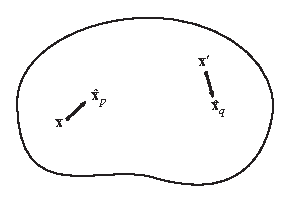
\includegraphics{../figures/chap04/fig01.eps}
\end{center}
\caption[seismorep]{\label{fig4.1}
无自转地球上的地震互易性:作用在~${\bf x}^{\prime}$~处~$\hat{\bf x}_q$~方向上的点力在~$\bf x$~处产生的响应的~$\hat{\bf x}_p$~分量等于作用在~$\bf x$~处~$\hat{\bf x}_p$~方向的点力在~${\bf x}^{\prime}$~处产生的响应的~$\hat{\bf x}_q$~分量。格林张量或单位脉冲响应的分量满足~$G_{pq}({\bf x},{\bf x}^{\prime};t)=G_{qp}
({\bf x}^{\prime},{\bf x};t)$。}
\end{wrapfigure}
~(\ref{4.reciprocity})~式所表达的是{\em 地震互易性原理}。笼统地讲,该原理表明,源点和接收点可以互换;要注意的是方向和位置必须对换,如图~\ref{fig4.1}~所示。
%%%

由于当~$\omega_k\rightarrow 0$~时,$\omega_k^{-1}\sin\omega_kt\rightarrow t$,因而地球的每一个平凡模式对格林张量~$\bG$~的贡献都随时间线性增长。这种线性增长并非意味着不稳定性,因为相应的质点速度~$\p_t\bG$~仍然是有界的。
无论如何,地震震源都不可能激发任何平凡模式。
\index{mode!trivial}%
\index{trivial mode}%
刚体模式是不能被激发的,因为没有任何内在源可以对地球施加净力或净力矩;地转模式也不能被激发,因为它们都局限于地球的液态区域,而地震皆发生在固态的地壳或地幔中。
\index{torque}%
\index{mode!geostrophic}%
\index{geostrophic mode}%
\index{mode!rigid-body}%
\index{rigid-body mode}%
我们称~(\ref{4.nrGreen})~的求和中扣除了平凡模式的~$\bG$~为{\em 地震格林张量}。
%%%
\index{Green tensor!seismic}%
\index{seismic Green tensor}%
\index{tensor!Green!non-rotating|)}%
\index{Green tensor!non-rotating Earth|)}%

%\subsection{Response to a transient force}
\subsection{对短时力的响应}
\index{transient force!non-rotating Earth|(}%
\index{force!transient|(}%

在第~5~章中,我们将展示任何内在源(如地震)都可以用作用在~$\earth$~上的等效体力密度~$\bef$~和作用在~$\p\earth$~上的等效面力密度~$\bt$~来表示。
\index{force!body}%
\index{body force}%
\index{force!surface}%
\index{surface force}%
任何这类源所产生的位移~$\bs$~均可写为脉冲响应~$\bG$~与等效力~$\bef$~和~$\bt$~在整个既往历程的卷积:
%%%
\eqa
\label{4.convol}
\lefteqn{
\bs(\bx,t)=\int_{-\infty}^t\int_{\subearth}\bG(\bx,\bx';t-t')\cdot\bef(\bx',t')
\,dV'\,dt'} \\
& & \mbox{}\qquad\qquad+\int_{-\infty}^t\int_{\partial\subearth}\bG(\bx,\bx';t-t')
\cdot\bt(\bx',t')\,d\/\Sigma'\,dt'. \nonumber
\ena
这一结果体现了叠加与因果原理,是不证自明的;对于有疑虑的读者,我们会在第~5.3~节中给出(在自转地球上的)推导。
%%%

将表达式~(\ref{4.nrGreen})~代入~(\ref{4.convol}),我们可以把~$\bs$~写成简正模式的叠加
%%%
\eq
\label{4.nrsxt1}
\bs(\bx,t)=\sum_{k}\omega_k^{-1}\bs_k(\bx)\int_{-\infty}^tA_k(t')\sin\omega_k(t-t')
\,dt',
\en
其中
%%%
\eq
\label{4.nrAkt1}
A_k(t)=\int_{\subearth}\bef(\bx,t)\cdot\bs_k(\bx)\,dV+
\int_{\spar\subearth}\bt(\bx,t)\cdot\bs_k(\bx)\,d\/\Sigma.
\en
对时间做分部积分,我们得到等价的结果
%%%
\eq
\label{4.nrsxt2}
\bs(\bx,t)=\sum_{k}\omega_k^{-2}\bs_k(\bx)\int_{-\infty}^t\p_{t'}
A_k(t')[1-\cos\omega_k(t-t')]\,dt',
\en
其中
%%%
\eq
\label{4.nrAkt2}
\p_tA_k(t)=\int_{\subearth}\p_t\bef(\bx,t)\cdot\bs_k(\bx)\,dV+
\int_{\spar\subearth}\p_t\bt(\bx,t)\cdot\bs_k(\bx)\,d\/\Sigma.
\en
公式~(\ref{4.nrsxt2})~将响应~$\bs$~表示为~Heaviside~或阶跃函数响应~$\omega_k^{-2}[1-\cos\omega_k(t-t')]$~的叠加,而~(\ref{4.nrsxt1})~则将其表示为狄拉克或脉冲响应~$\omega_k^{-1}\sin\omega_k(t-t')$~的叠加。
%%%
\begin{figure}[!b]
\begin{center}
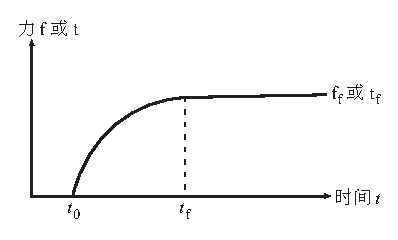
\includegraphics{../figures/chap04/fig02.eps}
\end{center}
\caption[transforce]{\label{fig4.2}
短时等效力~${\bf f}({\bf x},t)$~或~${\bf t}({\bf x},t)$~随时间变化示意图。等效力的起始时刻为~$t=t_0$,当~$t\geq t_{\rm f}$~时,分别达到稳态定值~${\bf f}({\bf x},t)$~或~${\bf t}({\bf x},t)$。}
\index{force!transient}%
\index{transient force}%
\end{figure}

与地震相关的等效力~$\bef$~和~$\bt$~在某一起始时刻~$t_0$~之前为零,而在~$t_{\rm f}$~之后分别达到恒定的静态值~$\bef_{\rm f}$~和~$\bt_{\rm f}$,如图~\ref{fig4.2}~所示。在第~5~章中,我们会看到,对于断层源,$t_{\rm f}-t_0$~这一时间段代表破裂的持续时间,而~$\bef_{\rm f}$~和~$\bt_{\rm f}$~这两个量则与断层上最终的静态滑动量有关。当~$t\geq t_{\rm f}$~时,等效力随时间的变化停止,对这种{\em 短时震源\/}的响应在形式上会特别简单。从~(\ref{4.nrsxt2})~式我们看到
%%%
\eq
\label{4.nrsxt3}
\bs(\bx,t)=\sum_k\omega_k^{-2}(a_k^{\rm f}-a_k\cos\omega_kt
-b_k\sin\omega_kt)_{\,}\bs_k(\bx),\quad t\geq t_{\rm f},
\en
其中
%%%
\eq
a_k^{\rm f}=\int_{\subearth}\bef_{\rm f}(\bx)\cdot\bs_k(\bx)\,dV+
\int_{\spar\subearth}\bt_{\rm f}(\bx)\cdot\bs_k(\bx)\,d\/\Sigma,
\en
\eqa
\lefteqn{
a_k=\int_{t_0}^{t_{\rm f}}\int_{\subearth}\p_t\bef(\bx,t)
\cdot\bs_k(\bx)\cos\omega_kt\,dV\,dt}
\nonumber \\
&&\mbox{}\qquad\qquad+
\int_{t_0}^{t_{\rm f}}\int_{\spar\subearth}\p_t\bt(\bx,t)
\cdot\bs_k(\bx)\cos\omega_kt\,d\/\Sigma\,dt,
\ena
\eqa
\lefteqn{
b_k=\int_{t_0}^{t_{\rm f}}\int_{\subearth}\p_t\bef(\bx,t)
\cdot\bs_k(\bx)\sin\omega_kt\,dV\,dt}
\nonumber \\
&&\mbox{}\qquad\qquad+
\int_{t_0}^{t_{\rm f}}\int_{\spar\subearth}\p_t\bt(\bx,t)
\cdot\bs_k(\bx)\sin\omega_kt\,d\/\Sigma\,dt.
\ena
对~(\ref{4.nrsxt3})~这一结果有很清楚的物理解释。振荡项~$a_k\cos\omega_kt$~和~$b_k\sin\omega_kt$~表示由地震所激发的地球的{\em 自由振荡\/}。
\index{free oscillations}%
地球内部不可避免存在的非弹性会导致这些振荡随时间衰减;因而在~$t\rightarrow \infty$~的极限时与时间无关的位移成为:
%%%
\eq
\label{4.nrsstat}
\bs_{\rm f}(\bx)=
\sum_k\omega_k^{-2}a_k^{\rm f}\bs_k(\bx).
\en
$\bs_{\rm f}$~表示地球对等效力的最终稳态值~$\bef_{\rm f}$~和~$\bt_{\rm f}$~的{\em 静态响应\/}。对于断层源,断层两侧的相对位错在地球内部各点~$\bx$~都产生一个永久形变。
%%%

在破裂停止后,质点的加速度~$\ba=\p_t^2\bs$~为
\index{acceleration}%
\index{particle acceleration}%
%%%
\eq
\label{4.nraxt}
\ba(\bx,t)=\sum_k(a_k\cos\omega_kt
+b_k\sin\omega_kt)_{\,}\bs_k(\bx),\quad t\geq t_{\rm f}.
\en
我们一般用加速度图来表示地球对地震的响应,因为这样可以简化后面章节中的一些理论结果。事实上,一个理想的加速度计除了对仪器外壳的加速度产生响应外,还会对地球的引力场的变化有所响应。我们将在第~4.4~节中讨论如何处理这些效应。
%%%
\index{transient force!non-rotating Earth|)}%
\index{force!transient|)}%
\index{normal mode!non-rotating Earth|)}%

\renewcommand{\thesection}{$\!\!\!\raise1.3ex\hbox{$\star$}\!\!$
\arabic{chapter}.\arabic{section}}
%\section{Rotating Earth Model}
\section{自转地球模型}
\index{normal mode!rotating Earth|(}%
\label{4.sec.rotmod}
\renewcommand{\thesection}{\arabic{chapter}.\arabic{section}}

自转地球在频率域的动量方程~(\ref{4.nrmodeqn})~为
%%%
\eqa
\label{4.rotmodeqn}
\lefteqn{
-\omega^2\rho^0\bs+2i\omega\rho^0\bOmega\times\bs-\bdel\cdot
\bT^{\rm PK1}}
\nonumber \\
&&\mbox{}\qquad\qquad+\rho^0\bdel\phi^{\rm E1}+\rho^0\bs\cdot\bdel\bdel
(\phi^0+\psi)=\bzero,
\ena
其中~$\psi$~是离心势函数。科里奥利力项~$2i\omega\rho^0\bOmega\times\bs$~的存在使得我们不能像对~(\ref{4.nrmodeqn})~的处理那样将~(\ref{4.rotmodeqn})~视为一个实的方程。自转地球模型的本征函数~$\bs$~{\em 本质上是复数的}。我们会继续假定本征频率~$\omega$~是实数(我们下面会证明任何久期稳定的地球模型都可确保这一点)。取~(\ref{4.rotmodeqn})~式的复共轭,我们注意到当且仅当~$\omega$、$\bs$~是本征解时,$-\omega$、$\bs^*$~也是本征解。这种成对的互为复共轭的本征解~$\omega$、$\bs$~与~$-\omega$、$\bs^*$~是自转地球简正模式的特性。
%%%

在相反方向自转的{\em 逆转地球\/}的本征频率和本征函数也是值得关注的。
\index{anti-Earth}%
注意到方程~(\ref{4.rotmodeqn})~在同时做~$\bOmega\rightarrow -\bOmega$~和~$\omega\rightarrow -\omega$~的变换时是不变的,我们看到当且仅当~$\omega$、$\bs$~是真实地球的模式时,$\omega$、$\bs^*$~也是逆转地球的模式。因此,本征频率~$\omega$~并不依赖于地球的自转方向。
%%%

\renewcommand{\thesubsection}{$\!\!\!\raise1.3ex\hbox{$\star$}\!\!$
\arabic{chapter}.\arabic{section}.\arabic{subsection}}
%\subsection{Orthonormality}
\subsection{正交归一性}
\index{orthonormality!rotating Earth|(}%
\label{4.sec.rotortho}
\renewcommand{\thesubsection}{\arabic{chapter}.\arabic{section}.\arabic{subsection}}

我们来重新定义自转地球的积分-微分算符~$\sH$,以便包含离心势函数~$\psi$:
\index{integro-differential operator}%
\index{operator!integro-differential}%
%%%
\eq
\label{4.rotHdef}
\rho^0\sH\bs=-\bdel\cdot\bT^{\rm PK1}+\rho^0\bdel\phi^{\rm E1}
+\rho^0\bs\cdot\bdel\bdel(\phi^0+\psi).
\en
从而频率域的动量方程~(\ref{4.rotmodeqn})~以及边界条件~(\ref{4.bc1})--(\ref{4.bc4})~可以用符号形式写为
%%%
\eq
\label{4.rotHeqn}
\sH\bs+2i\omega\bOmega\times\bs=\omega^2\bs.
\en
方程~(\ref{4.rotHeqn})~是一个非标准本征值问题,因为本征频率~$\omega$~在科里奥利项~$2i\omega\bOmega\times\bs$~中是线性的,而在惯性项~$\omega^2\bs$~中是二次的。
%%%

我们定义自转地球~$\earth$~中任意两个复函数~$\bs$~和~$\bs'$~的{\em 内积\/}为
\index{inner product!rotating Earth}%
%%%
\eq
\label{4.inprod2}
\langle\bs,\bs'\rangle=\int_{\subearth}\rho^0\bs^*\cdot\bs'\,dV.
\en
很容易验证~(\ref{4.rotHeqn})~中的算符~$\sH$~与~$i\bOmega\times$~在~(\ref{4.inprod2})~的复内积定义下具有{\em 厄米特\/}或{\em 自共轭\/}性质:
\index{Hermitian operator}%
\index{operator!Hermitian}%
\index{self-adjoint operator}%
\index{operator!self-adjoint}%
%%%
\eq
\label{4.rotHERM}
\langle\bs,\sH\bs'\rangle=\langle\sH\bs,\bs'\rangle
=\langle\bs',\sH\bs\rangle^*,
\en
\eq
\label{4.rotHERM2}
\langle\bs,i\bOmega\times\bs'\rangle=\langle i\bOmega\times\bs,\bs'\rangle
=\langle\bs',i\bOmega\times\bs\rangle^*.
\en
要建立~(\ref{4.rotHERM})~式可以直接将验证无自转地球的~(\ref{4.HERM})~式所做的推导加以拓展,而~(\ref{4.rotHERM2})~式则是简单的三重积等式。方程~(\ref{4.rotHeqn})~的厄米特性质应该并不意外---在有没有自转的地球模型中能量都是守恒的,正如我们在第~3.8~节中所见。
%%%

取~$\sH\bs+2i\omega \bOmega\times\bs=\omega^2\bs$~与~$\bs'$~的内积得到
%%%
\eq
\label{4.rotnew1}
\label{4.firstint}
\omega^2\langle\bs',\bs\rangle-2\omega\langle\bs',
i\bOmega\times\bs\rangle-\langle\bs',\sH\bs\rangle=0, 
\en
而取~$\sH\bs'+2i\omega' \bOmega\times\bs'=\omega^{\prime 2}\bs'$~与~$\bs$~的内积则有
%%%
\eq
\label{4.secint}
\omega^{\prime 2}\langle\bs,\bs'\rangle-2\omega'\langle\bs,
i\bOmega\times\bs'\rangle-\langle\bs,\sH\bs'\rangle=0.
\en
从~(\ref{4.secint})~中减去~(\ref{4.firstint}),并利用厄米特对称性~(\ref{4.rotHERM})--(\ref{4.rotHERM2})~式,我们得到
%%%
\eq
\label{4.rotORTHO}
\langle\bs,\bs'\rangle-2(\omega+\omega')
^{-1}\langle\bs,i\bOmega\times\bs'\rangle=0
\quad\mbox{当}\quad\omega\neq\omega',
\en
这里为方便起见,我们已经除以本征频率之和~$\omega+\omega'$。与~(\ref{4.NORMAL})~对应,~(\ref{4.rotORTHO})~是自转弹性地球中简正模式{\em 正交性\/}的表达式。
\index{orthogonality!rotating Earth}%
具有不同的正本征频率~$\omega\not =\omega'$~的复本征函数~$\bs$~和~$\bs'$~在~$\langle\bs,\bs'\rangle=0$~这一通常的意义上并不是正交的;相反地,正交性条件明确地涉及科里奥利项。对于本征函数的{\em 归一化\/},我们要求
%%%
\eq
\label{4.rotNORM}
\langle\bs,\bs\rangle-\omega
^{-1}\langle\bs,i\bOmega\times\bs\rangle=1.
\en
\index{normalization condition!rotating Earth}%
有了这一选择,在~$\bOmega=\bzero$~的无自转的极限情形,正交归一性关系~(\ref{4.rotORTHO})--(\ref{4.rotNORM})~退化为之前的~(\ref{4.NORMAL})--(\ref{4.ANORMAL})。
%%%
\index{orthonormality!rotating Earth|)}%

\renewcommand{\thesubsection}{$\!\!\!\raise1.3ex\hbox{$\star$}\!\!$
\arabic{chapter}.\arabic{section}.\arabic{subsection}}
%\subsection{Reduction to a standard eigenvalue problem}
\subsection{转化为标准本征值问题}
\renewcommand{\thesubsection}{\arabic{chapter}.\arabic{section}.\arabic{subsection}}

遵循~\textcite{dyson&schutz79}~和~\textcite{wahr81a},我们可以将非标准本征值问题~(\ref{4.rotHeqn})~转化为普通的本征值问题,其代价是本征函数的维数翻倍。我们将一个{\em 六维\/}矢量
%%%
\index{vector!six-dimensional}%
\eq
\bz=\left(\begin{array}{c}
\bs \\ \omega\bs
\end{array}\right)
\en
赋予每一个三维本征函数~$\bs$~和本征频率~$\omega$。很容易证明~(\ref{4.rotHeqn})~等价于
%%%
\eq
\label{4.rotKeqn}
\sK\bz=\omega\bz,
\en 
%%%
其中
%%%
\eq
\label{4.rotKdef}
\sK=\left(\begin{array}{cc}
0 & 1 \\ \sH & 2i\bOmega\,\times
\end{array}\right).
\en
因此,$\omega$~和~$\bz$~可以被视为六维线性算子~$\sK$~的本征频率和相应的本征函数。
%%%

对任意两个六维矢量
\eq
\bz=\left(\begin{array}{c}
\bs \\ \bv
\end{array}\right),\qquad
\bz'=\left(\begin{array}{c}
\bs' \\ \bv'
\end{array}\right)
\en
我们定义其点积或标量积为~$\bz\cdot\bz'=\bs\cdot\bs'+\bv\cdot\bv'$,而其{\em 内积\/}~$\langle_{\!}\langle\bz,\bz'\rangle_{\!}\rangle$~则定义为
\index{inner product!six-vector}%
\eq
\label{4.rotinprod}
\langle_{\!}\langle\bz,\bz'\rangle_{\!}\rangle=\int_{\subearth}
\bz^*\cdot\sP\bz'\,dV,
\en
其中
%%%
\eq
\sP=\rho^0\left(\begin{array}{cc}
\sH & 0 \\  0 & 1
\end{array}\right).
\en
用相应的三维矢量以显示写开来,该六维内积为~$\langle_{\!}\langle\bz,\bz'\rangle_{\!}\rangle=\langle\bs,\sH\bs'\rangle+\langle\bv,\bv'\rangle$。如果~$\bz$~和~$\bz'$~均为六维本征函数,即~$\bv=\omega\bs$~且~$\bv'=\omega'\bs'$,
那么我们有~$\langle_{\!}\langle\bz,\bz'\rangle_{\!}\rangle=\langle\bs,\sH\bs'\rangle
+\omega\omega'\langle\bs,\bs'\rangle$。
%%%

在六维内积~(\ref{4.rotinprod})~定义下,算子~$\sK$~在形式上是{\em 自共轭的\/}或{\em 厄米特的\/},即对于任意两个六维矢量~$\bz$~和~$\bz'$
\index{self-adjoint operator}%
\index{Hermitian operator}%
\index{operator!self-adjoint}%
\index{operator!Hermitian}%
%%%
\eq
\label{4.sixHERM}
\langle_{\!}\langle\bz,\sK\bz'\rangle_{\!}\rangle=
\langle_{\!}\langle\sK\bz,\bz'\rangle_{\!}\rangle=
\langle_{\!}\langle\bz',\sK\bz\rangle_{\!}\rangle^*
\en
通过简单的运算可以证明上述关系;$\langle_{\!}\langle\bz,\sK\bz'\rangle_{\!}\rangle$~和~$\langle_{\!}\langle\bz',\sK\bz\rangle_{\!}\rangle$~两者由下式明确给定:
%%%
\eq
\label{4.proof}
\langle_{\!}\langle\bz,\sK\bz'\rangle_{\!}\rangle=
\int_{\subearth}\rho^0\left[\left( \begin{array}{cc}
\bs & \bv \end{array} \right)^* \cdot \left( \begin{array}{cc}
0 & \sH \\ \sH & 2i\bOmega\,\times \end{array} \right) \left( \begin{array}{c}
\bs' \\ \bv' \end{array} \right) \right] dV,
\en
\eq
\label{4.proof2}
\langle_{\!}\langle\bz',\sK\bz\rangle_{\!}\rangle=
\int_{\subearth}\rho^0\left[\left( \begin{array}{cc}
\bs' & \bv' \end{array} \right)^* \cdot \left( \begin{array}{cc}
0 & \sH \\ \sH & 2i\bOmega\,\times \end{array} \right) \left( \begin{array}{c}
\bs \\ \bv \end{array} \right) \right] dV,
\en
这里我们使用了算子等式:
%%%
\eq
\label{4.PKdef}
\sP\sK=
\rho^0\left(\begin{array}{cc}
\sH & 0 \\  0 & 1
\end{array}\right)
\left(\begin{array}{cc}
0 & 1 \\ \sH & 2i\bOmega\,\times
\end{array}\right)
=\rho^0\left( \begin{array}{cc}
0 & \sH \\ \sH & 2i\bOmega\,\times \end{array} \right).
\en
执行~(\ref{4.proof})~和~(\ref{4.proof2})~中所显示的运算,再把结果用三维内积表示,我们得到
%%%
\eq
\label{4.proof3}
\langle_{\!}\langle\bz,\sK\bz'\rangle_{\!}\rangle=
\langle\bs,\sH\bv'\rangle+\langle\bv,\sH\bs'\rangle
+2\langle\bv,i\bOmega\times\bv'\rangle,
\en
\eq
\label{4.proof4}
\langle_{\!}\langle\bz',\sK\bz\rangle_{\!}\rangle=
\langle\bs',\sH\bv\rangle+\langle\bv',\sH\bs\rangle
+2\langle\bv',i\bOmega\times\bv\rangle.
\en
根据厄米特对称性~(\ref{4.rotHERM})--(\ref{4.rotHERM2}),~(\ref{4.proof3})~等于~(\ref{4.proof4})~的复共轭;由此建立了六维厄米特关系~(\ref{4.sixHERM})。从根本上说,是~$\sH$~和~$i\bOmega\times$~的厄米特性质决定了算子~$\sK$~的自共轭性。
%%%

取~$\sK\bz=\omega\bz$~与~$\bz'$~以及~$\sK\bz'=\omega'\bz'$~与~$\bz$~的六维内积,并将结果相减,我们得到六维正交关系
%%%
\index{orthogonality!rotating Earth}%
\eq
\label{4.rotortho2}
\langle_{\!}\langle\bz,\bz'\rangle_{\!}\rangle=0
\quad\mbox{当}\quad\omega\neq\omega'.
\en
很容易验证~(\ref{4.rotortho2})~与三维正交关系~(\ref{4.rotORTHO})~是等价的;用~(\ref{4.firstint})~消去~$\langle\bs,\sH\bs'\rangle$,我们看出~$\langle_{\!}\langle\bz,\bz'\rangle_{\!}\rangle=\omega(\omega+\omega')
[\langle\bs,\bs'\rangle-2(\omega+\omega')^{-1}
\langle\bs,i\bOmega\times\bs'\rangle]$。
与~(\ref{4.rotNORM})~等价的六维归一化条件为
%%%
\eq
\label{4.newNORM}
\langle_{\!}\langle\bz,\bz\rangle_{\!}\rangle=2\omega^2.
\en
因此,自转地球中涉及科里奥利力的非常规的正交归一性关系被视为是六维本征函数空间中的一般正交归一性关系。
%%%

上面的推导尽管优雅,却有一个小缺陷:(\ref{4.rotinprod})~这一关系并没有在由地球模型~$\earth$~中所有分段光滑的六维矢量~$\bz$~组成的空间中定义一个合理的内积,因为存在一类六维范数~$\langle_{\!}\langle\bz,\bz\rangle_{\!}\rangle$~为零的平凡模式。解决该问题的方法很简单---我们只需从所考虑的空间中剔除平凡模式以及任何其它同样不满足约束条件~$\langle_{\!}\langle\bz,\bz
\rangle_{\!}\rangle > 0$~的相关矢量;
\index{trivial mode}%
\index{mode!trivial}%
这一剔除步骤的技术细节可参见~\textcite{wahr81a}。在第~4.2.5节~和第~4.2.7--4.2.8~节,我们以平凡模式为例,简要描述在简正模式的激发问题中它们是如何被处理的。
%%%

\renewcommand{\thesubsection}{$\!\!\!\raise1.3ex\hbox{$\star$}\!\!$
\arabic{chapter}.\arabic{section}.\arabic{subsection}}
%\subsection{Rayleigh's principle}
\subsection{瑞利原理}
\label{4.sec.rotRay}
\index{Rayleigh's principle!rotating Earth|(}%
\renewcommand{\thesubsection}{\arabic{chapter}.\arabic{section}.\arabic{subsection}}

瑞利原理可以很容易推广到自转地球模型。取~$\sK\bz=\omega\bz$~与~$\bz$~的六维内积,我们得到{\em 瑞利商\/}:
%%%
\index{Rayleigh quotient!rotating Earth}%
\eq
\label{4.sixRayquo}
\omega=\frac{\langle_{\!}\langle\bz,\sK\bz\rangle_{\!}\rangle}
{\langle_{\!}\langle\bz,\bz\rangle_{\!}\rangle}.
\en
我们视~(\ref{4.sixRayquo})~的右侧为一个泛函,对每一个非零的六维矢量~$\bz$~它都赋予一个标量~$\omega$。瑞利原理指出,当且仅当~$\bz$~为与本征频率~$\omega$~相关的算子~$\sK$~的本征函数时,该泛函对于任意变化~$\bdelta\bz$~是稳定的。要验证这一点,我们看到当精确到~$\|\bdelta\bz\|$~的一阶时有
%%%
\eqa
\label{4.deltaom}
\lefteqn{\delta\omega=\frac{\langle_{\!}\langle\bdelta\bz,\sK\bz\rangle_{\!}\rangle
+\langle_{\!}\langle\bz,\sK\bdelta\bz\rangle_{\!}\rangle
-\omega\langle_{\!}\langle\bdelta\bz,\bz\rangle_{\!}\rangle
-\omega\langle_{\!}\langle\bz,\bdelta\bz\rangle_{\!}\rangle}
{\langle_{\!}\langle\bz,\bz\rangle_{\!}\rangle}} \nonumber \\
& & \mbox{}\hspace{-2.9 mm}=\frac{2_{\,}\Re{\rm e}_{\,}
\langle_{\!}\langle\bdelta\bz,\sK\bz-\omega\bz
\rangle_{\!}\rangle}{\langle_{\!}\langle\bz,\bz\rangle_{\!}\rangle},
\ena
这里我们使用了算子~$\sK$~的自共轭性。从~({\ref{4.deltaom})~这一结果可以清楚地看到,当且仅当~$\omega$~和~$\bz$~满足~$\sK\bz=\omega\bz$~时,对任意的~$\bdelta\bz$,$\delta\omega$~均为零。由此我们建立了六维形式的瑞利原理。

与此等价,作为稳定泛函我们也可以不用本征频率~$\omega$,而是考虑{\em 作用量}
\index{action}%
\eq
\label{4.sixact}
\sI=\half\langle_{\!}\langle
\bz,\bz\rangle_{\!}\rangle-\half\omega^{-1}
\langle_{\!}\langle\bz,\sK\bz\rangle_{\!}\rangle
\en
精确到~$\|\bdelta\bz\|$~的一阶,$\sI$~的变分为
\eq
\delta\sI=\omega^{-1}\Re{\rm e}_{\,}
\langle_{\!}\langle\bdelta\bz,\omega\bz-\sK\bz
\rangle_{\!}\rangle,
\en
这里我们再次用到了~$\sK$~的自共轭性。显然,$\delta\omega$~和~$\delta \sI$~这两个变化通过~$\delta\omega=-2\omega\langle_{\!}\langle\bz,\bz\rangle_{\!}\rangle^{-1}\delta\sI$~联系起来,因而瑞利商~$\om$~和作用量~$\sI$~具有共同的稳定点~$\bz$。

作用量~$\sI$~也可以用三维本征函数~$\bs$~表示为
\eq
\label{4.threeact}
\sI=\half
\omega^2\langle\bs,\bs\rangle-\omega\langle\bs,i\bOmega\times\bs\rangle
-\half\langle\bs,\sH\bs\rangle.
\en
(\ref{4.threeact})~是~(\ref{4.firstact})~的自然推广,要得到这一结果,需要在六维定义式~(\ref{4.sixact})~中引入因子~$\omega^{-1}$。由位移场的一个无穷小变化~$\bdelta\bs$~所引起的~$\sI$~的变分为
\eq
\label{4.threeact2}
\delta\sI=\Re{\rm e}_{\,}\langle\bdelta\bs,\omega^2\bs-2i\omega\bOmega
\times\bs-\sH\bs\rangle,
\en
这里我们使用了算子~$\sH$~和~$i\bOmega\times$~的自共轭性~(\ref{4.rotHERM})--(\ref{4.rotHERM2})。从~(\ref{4.threeact2})~可以清楚看到,当且仅当~$\sH\bs+2i\omega\bOmega\times\bs=\omega^2\bs$~时,对于任意变化~$\bdelta\bs$,$\delta\sI$~均为零;这是瑞利原理的一种不同的三维表述。

同无自转情形一样,以上示意性的“证明”在与算子~$\sH$~相关的边界条件以及变化~$\bdelta\bs$~所必须满足的可容许性条件上过于随意。要做更严格的推导,我们将三维作用量~(\ref{4.threeact})~重新写为
\eq
\label{4.ACTION}
\sI=\half(\omega^2\sT-2\omega\sW-\sV),
\en
其中
\eq
\label{4.rotTdef}
\sT=\int_{\subearth}\rho^0\bs^*\cdot\bs\,dV,
\en
\eq
\label{4.Wdef}
\sW=\int_{\subearth}\rho^0\bs^*\cdot(i\bOmega\times\bs)\,dV,
\en
\vspace{-3 mm}
\eqa
\label{4.rotVdef}
\lefteqn{\sV=\int_{\subearth}
[\bdel\bs^*\!:\!\bLambda\!:\!\bdel\bs
+\half\rho^0(\bs^*\cdot\bdel\phi^{\rm E1}
+\bs\cdot\bdel\phi^{{\rm E1}\ast})} \nonumber \\
&&\mbox{}\qquad+\rho^0
\bs^*\cdot\bdel\bdel(\phi^0+\psi)\cdot\bs]\,dV \nonumber \\
&&\mbox{}+\half\int_{\Sigma_{\rm FS}}[\varpi^0\bs^*
\cdot(\bdel^{\Sigma}\bs)\cdot\bnh
+\varpi^0\bs\cdot(\bdel^{\Sigma}\bs^*)\cdot\bnh \nonumber \\
&&\mbox{}\qquad-(\bnh\cdot\bs^*)\bdel^{\Sigma}\cdot(\varpi^0\bs)
-(\bnh\cdot\bs)\bdel^{\Sigma}\cdot(\varpi^0\bs^*)]^+_-\,d\/\Sigma.
\ena
我们分别称~$\sT$、$\sW$~和~$\sV$~为{\em 动能泛函\/}、{\em 科里奥利泛函\/}和{\em 势能泛函\/}。
\index{functional!kinetic energy}%
\index{kinetic energy functional}%
\index{functional!Coriolis}%
\index{Coriolis functional}%
\index{functional!potential energy}%
\index{potential energy functional}%
动能和势能泛函的定义方式与无自转地球的~(\ref{4.Tdef})~和~(\ref{4.Vdef})~类似,不同之处在于我们容许复数的本征函数~$\bs$,且将引力势函数~$\phi^0$~换为重力势函数~$\phi^0+\psi$。(\ref{4.rotTdef})--(\ref{4.rotVdef})~这三个泛函均为自变量~$\bs$~的实的二次函数,因而作用量~$\sI$~亦然。

{\em 位移形式的\/}瑞利原理表明,
\index{variational principle!displacement}%
当且仅当~$\bs$~是本征频率为~$\omega$~的本征函数时,对于任意可容许变化~$\bdelta\bs$,$\sI$~是稳定的。如同第~\ref{4.sec.Rayprin}~节中所做的,应用三维和二维形式的高斯定理,我们得到
\eqa
\label{4.deltaIrot2}
\lefteqn{
\delta\sI=\Re{\rm e}\int_{\subearth}\bdelta\bs^*\cdot[\omega^2\rho^0\bs
-2i\omega\rho^0\bOmega\times\bs+\bdel\cdot\bT^{\rm PK1}} \nonumber \\
&&\mbox{}\qquad\qquad-\rho^0\bdel
\phi^{\rm E1}-\rho^0\bs\cdot\bdel\bdel
(\phi^0+\psi)]\,dV \nonumber \\
& & \mbox{}-\Re{\rm e}\int_{\partial\subearth}\bdelta\bs^*\cdot(\bnh\cdot\bT^{\rm PK1})
\,d\/\Sigma \nonumber \\
& & \mbox{}+\Re{\rm e}\int_{\Sigma_{\rm SS}}\bdelta\bs^*\cdot[\bnh\cdot\bT^{\rm PK1}]^+_-
\,d\/\Sigma \nonumber \\
& & \mbox{}
+\Re{\rm e}\int_{\Sigma_{\rm FS}}[\bdelta\bs^*\cdot\bt^{\rm PK1}]^+_-\,d\/\Sigma.
\ena
(\ref{4.deltaIrot2})~式显示,当且仅当本征频率~$\omega$~及相应本征函数~$\bs$~满足自转地球的简正模式方程~(\ref{4.rotmodeqn})~以及动力学边界条件~(\ref{4.bc1})--(\ref{4.bc4})~时,对于任意可容许变化~$\bdelta\bs$,$\delta\sI=0$,这正是瑞利原理所说的。

自转地球当然也有其{\em 位移-势函数形式\/}的瑞利原理。
\index{variational principle!displacement-potential}%
以类似于~(\ref{4.Vdef2})~的方式,容许复数的本征函数,并将~$\phi^0$~换为~$\phi^0+\psi$,我们定义修改后的势能泛函~$\sV'$:
\eqa
\label{4.Vmodrot}
\lefteqn{\sV'
=\int_{\subspace} [\bdel\bs^*\!:\!\bLambda\!:\!\bdel\bs
+\rho^0(\bs^*\cdot\bdel\phi^{\rm E1}
+\bs\cdot\bdel\phi^{{\rm E1}\ast})} \nonumber \\
&&\mbox{}\qquad+\rho^0
\bs^*\cdot\bdel\bdel(\phi^0+\psi)\cdot\bs
+(4\pi G)^{-1}\bdel\phi^{{\rm E1}
\ast}\cdot\bdel\phi^{\rm E1}]\,dV \nonumber \\
&&\mbox{}+\half\int_{\Sigma_{\rm FS}}
[\varpi^0\bs^*\cdot(\bdel^{\Sigma}\bs)\cdot\bnh
+\varpi^0\bs\cdot(\bdel^{\Sigma}\bs^*)\cdot\bnh \nonumber \\
&&\mbox{}\qquad-(\bnh\cdot\bs^*)\bdel^{\Sigma}\cdot(\varpi^0\bs)
-(\bnh\cdot\bs)\bdel^{\Sigma}\cdot(\varpi^0\bs^*)]^+_-\,d\/\Sigma.
\ena
当且仅当~$\omega$、$\bs$、$\phi^{\rm E1}$~为一本征解时,对于任意且独立的可容许变化~$\bdelta\bs$~和~$\delta\phi^{\rm E1}$,其相应的修改后的作用量
\eq
\label{4.needACTION}
\sI'=\half(\omega^2\sT-2\omega\sW-\sV')
\en
是稳定的。由于等式~(\ref{3.twoints}),对于任意本征解,$\sV$~与~$\sV'$~这两个势能泛函以及~$\sI$~与~$\sI'$~这两个作用量都是相等的。由于~(\ref{4.sixRayquo})~和~(\ref{4.sixact}),作用量的稳定值为
\eq \label{3.zeroact}
\sI=\sI'=0,
\en
要得到~(\ref{3.zeroact})~这一结果也可以将三维动量方程~(\ref{4.rotmodeqn})~与~$\bs^*$~点乘,并在地球模型~$\earth$~上积分,或者等价地,在~(\ref{4.firstint})~和~(\ref{4.secint})~两式中令带撇号与不带撇号的本征解相等。

$\sI$~和~$\sI'$~的稳定性也可以直接用哈密顿原理推出,对固定的频率~$\omega$,考虑时间域位移:
\eq
\label{4.realcycle}
\bs(\bx,t)=\half[\bs(\bx)\exp(i\omega
t)+\bs^*(\bx)\exp(-i\omega t)],
\en
如果时间间隔~$t_2-t_1$~是振荡周期的整数倍,则时间域的作用量~(\ref{3.action})~和~(\ref{3.action3})~分别为常数乘以~(\ref{4.ACTION})~和~(\ref{4.needACTION}),因而瑞利原理是哈密顿原理的特例。要注意的是~(\ref{3.sTdef})--(\ref{3.sVdef})~中的瞬时相对动能和弹性-引力势能与~(\ref{4.rotTdef})~和~(\ref{4.rotVdef})~中的不依赖时间的泛函~$\sT$~和~$\sV$~之间的区别。从物理上讲,泛函~$\omega^2\sT$~和~$\sV$~是以~(\ref{4.realcycle})~形式振荡的相对动能和势能在一个周期上的{\em 平均值的四倍\/}。
\index{Rayleigh's principle!rotating Earth|)}%

\renewcommand{\thesubsection}{$\!\!\!\raise1.3ex\hbox{$\star$}\!\!$
\arabic{chapter}.\arabic{section}.\arabic{subsection}}
%\subsection{Dynamical stability}
\subsection{动力学稳定性}
\index{stability!dynamical!rotating Earth|(}%
\index{dynamical stability!rotating Earth|(}%
\renewcommand{\thesubsection}{\arabic{chapter}.\arabic{section}.\arabic{subsection}}

将能量平衡关系~$\omega^2\sT-2\omega\sW-\sV=0$~视为一个~$\omega$~的二次方程,我们看到与本征函数~$\bs$~相关的本征频率必须是下面的两个解之一
\eq
\label{4.quadsol}
\omega=\frac{\sW\pm\sqrt{\sW^2+\sT\sV}}
{\sT}.
\en
因为~$\sW^2\geq 0$~且~$\sT > 0$,本征频率均为实数,因此,只要对~$\earth$~中所有分段光滑函数~$\bs$ 都有
\eq
\label{4.Vnonneg}
\sV\geq 0,
\en
地球就是动力学稳定的。
(\ref{4.Vnonneg})~是第~3.9.6~节中得到的久期稳定的条件,同时我们看到久期稳定性意味着动力学稳定性。然而,$\sV\geq 0$~在此并不是动力学稳定性必要和充分条件;这里的必要条件是只要公式~(\ref{4.quadsol})~中的判别式~$\sW^2+\sT\sV$~为非负即可,而即便是~$\sV<0$,即初始构形的弹性-引力势能是局部的极大值而非局部的极小值,这个必要条件也是能够被满足的。这种动态稳定但久期不稳定构形的一个经典例子是绕最小惯量主轴自转的准刚性地球模型。在没有任何摩擦耗散时,一个小扰动就会激发一个稳定的欧拉自由章动或钱德勒摆动。然而,如果存在任何的非弹性,该振荡的振幅将以一个取决于能量耗散的速率而增大,并且地球将重新定向,直到自转轴与最大惯量主轴重叠。绕最大惯量主轴均匀自转是角动量固定的地球模型唯一的久期稳定构形;这一状态的小扰动会激发一个衰减的钱德勒摆动。因而我们自此将假设地球在地震之前处于这种
久期稳定状态,即对所有可能的弹性-引力形变均有~$\sV\geq 0$。
\index{Chandler wobble}%
\index{nutation}%
\index{stability!dynamical!rotating Earth|)}%
\index{dynamical stability!rotating Earth|)}%

\renewcommand{\thesubsection}{$\!\!\!\raise1.3ex\hbox{$\star$}\!\!$
\arabic{chapter}.\arabic{section}.\arabic{subsection}}
%\subsection{Rigid-body and geostrophic modes}
\subsection{刚体模式与地转模式}
\index{mode!rigid-body|(}%
\index{mode!geostrophic|(}%
\index{rigid-body mode|(}%
\index{geostrophic mode|(}%
\label{4.sec.rottriv}
\renewcommand{\thesubsection}{\arabic{chapter}.\arabic{section}.\arabic{subsection}}

自转地球的平凡模式由六维范数~$\langle_{\!}\langle\bz,\bz'\rangle_{\!}\rangle$ 为零的本征解组成;
\index{trivial mode}%
\index{mode!trivial}%
用三维动能和势能泛函表示的相应的条件为~$\sV+\omega^2\sT=0$。与无自转地球一样,有两类平凡模式:整个地球的刚体模式和仅限于液态区域~$\earth_{\rm F}$的地转模式。
%%%

自转地球的刚体模式比无自转地球的要更复杂;但是,从根本上讲,它们仍然来自刚体运动的六个自由度。要列举这些模式,采用~$\bzh$~与自转轴~$\bOmega=\Omega\bzh$~平行,从而使$\bxh$~和~$\byh$~采用在赤道面上的笛卡尔坐标系更为方便。{\em 轴向平动模式\/}的本征频率和未归一化本征函数为
\index{rotation axis}%
\index{axis!of rotation}%
\index{mode!axial translational}%
\index{axial translational mode}%
\eq
\label{4.axtrans}
\omega=0,\qquad\bs=\bzh,
\en
而轴向转动模式则有
\eq
\label{4.axspin}
\omega=0,\qquad\bs=\bzh\times\bx.
\en
(\ref{4.axtrans})~和~(\ref{4.axspin})~分别对应于与自转轴方向平行的刚体平动和绕自转轴的刚体自转。而两个{\em 赤道面平动模式\/}的本征解为:
\index{rotation axis}%
\index{axis!of rotation}%
\index{equatorial translational mode}%
\index{mode!equatorial translational}%
\eq
\label{4.eqtrans}
\omega=\pm\Omega,\qquad\bs=\bxh\pm i\byh.
\en
此时的运动包括在惯性参照系中平行于赤道面的恒定平动;在转动参照系中,这一恒定位移以一个表观的周日运动呈现。最后一个能够解析给定的刚体模式是{\em 倾斜模式\/},其本征解为
\index{tilt-over mode}%
\index{mode!tilt-over}%
\eq
\label{4.tiltover}
\omega=\pm\Omega,\qquad\bs=(\bxh\pm i\byh)\times\bx.
\en
该模式对应于一个赤道面的恒定转动,或者是地球在惯性参照系中相对于自转轴的倾斜;在地面观测者的参照系中(即转动参照系中),它也是以一个周日运动呈现出来。(\ref{4.axtrans})--(\ref{4.tiltover})~中的所有位移场都是零应变的,即$\beps=\bzero$,因此相应的密度和引力势函数的欧拉微扰都是纯平流的:即$\rho^{\rm E1}=-\bs\cdot\bdel\rho^0$,$\phi^{\rm E1}=-\bs\cdot\bdel\phi^0$。弹性引力算子~(\ref{4.rotHdef})~简化为~$\rho^0\sH\bs=\rho^0\bs\cdot\bdel\bdel\psi-\rho^0\bdel\psi\cdot\bdel\bs$,因而满足了方程~(\ref{4.rotHeqn})。对于两个赤道面平动模式,判别式~$\sW^2+\sT\sV$~均为零,因此它们
占有了两个赤道面平动自由度。另一方面,倾斜模式仅占有赤道面转动自由度中的一个;另一个赤道面转动模式是钱德勒摆动~(Smith \& Dahlen \citeyear{smith&dahlen81})。前四个刚体模式~(\ref{4.axtrans})--(\ref{4.eqtrans})~均有~$\langle_{\!}\langle \bz,\bz\rangle_{\!}\rangle=0$;因此,在用~(\ref{4.rotinprod})~作为内积之前,必须将它们从可容许的六维矢量空间中剔除。倾斜模式~(\ref{4.tiltover})~并不是平凡模式,因为它有~$\langle_{\!}\langle
\bz,\bz\rangle_{\!}\rangle=2C\Omega^2$,其中~$C$~是地球的球极转动惯量(即主转动惯量)。

地转模式在特征上与无自转地球的完全一样;其相应的位移本征函数~$\bs$~的形式为~(\ref{4.geostr1})--(\ref{4.geostr2}),本征频率为~$\omega=0$。唯一的区别是~$\rho^0$~和~$p^0$~的等值面与重力势函数~$\phi^0+\psi$~而不是~$\phi^0$~自身的等值面重合。如第~4.1.6~节所讨论的,在任何中立分层的~$\earth_{\rm F}$~区域内,地转流的家族更大。一般而言,地转模式的本征空间包含~$\earth_{\rm F}$~中不改变地球弹性-引力势能~$\sV$~的所有稳定流。
\index{mode!rigid-body|)}%
\index{mode!geostrophic|)}%
\index{rigid-body mode|)}%
\index{geostrophic mode|)}%

\renewcommand{\thesubsection}{$\!\!\!\raise1.3ex\hbox{$\star$}\!\!$
\arabic{chapter}.\arabic{section}.\arabic{subsection}}
%\subsection{Green tensor}
\subsection{格林张量}
\index{Green tensor!rotating Earth|(}%
\index{tensor!Green!rotating|(}%
\label{4.sec.rotGreen}
\renewcommand{\thesubsection}{\arabic{chapter}.\arabic{section}.\arabic{subsection}}

自转地球的格林张量或脉冲响应~$\bG(\bx,\bx';t)$~满足齐次方程
\eq
\label{4.rotGreen}
\rho^0(\p_t^2\bG+2i\bOmega\times\p_t\bG+\sH\bG)=\bzero,
\en 
连同初始条件
\eq
\label{4.rotGreenic}
\bG(\bx,\bx';0)=\bzero,\qquad\p_t\bG(\bx,\bx';0)=(1/_{\!}\rho^0)\bI_{\,}\delta(\bx-\bx').
\en
若要求解~(\ref{4.rotGreen})--(\ref{4.rotGreenic}),我们假设本征函数~$\bs_k$~及其复共轭~$\bs_k^*$~构成一个完备集,并将~$\bG$~写为
\index{completeness}%
\eq
\bG(\bx,\bx';t)=\Re{\rm e}\sum_k\bs_k(\bx)\bc_k(\bx')\exp(i\omega_kt).
\en
要使这一展开式满足初始条件~(\ref{4.rotGreenic})~的前提是
\eq
\label{4.rotck1}
\sum_k(\bs_k\bc_k+\bs_k^*\bc_k^*)=\bzero,
\en
\eq
\label{4.rotck2}
\sum_k(\omega_k\bs_k\bc_k-\omega_k\bs_k^*\bc_k^*)=
-(2i/_{\!}\rho^0)\bI_{\,}\delta(\bx-\bx').
\en
我们可以将~(\ref{4.rotck1})--(\ref{4.rotck2})~在六维本征函数空间中写为单个方程:
\eq
\label{4.rotck3}
\sum_k(\bz_k\bc_k+\bz_k^*\bc_k^*)=
\left(\begin{array}{c}
\bzero \\ -(2i/_{\!}\rho^0)\bI_{\,}\delta(\bx-\bx')
\end{array}\right),
\en
其中
\eq
\bz_k=\left(\begin{array}{c}
\bs_k \\ \omega_k\bs_k
\end{array}\right),\qquad
\bz_k^*=\left(\begin{array}{c}
\bs_k^* \\ -\omega_k\bs_k^*
\end{array}\right).
\en
取~(\ref{4.rotck3})~与~$\bz_{k'}$~和~$\bz_{k'}^*$~的六维内积,并利用正交归一关系~$\langle_{\!}\langle\bz_k,\bz_{k'}\rangle_{\!}\rangle
=2\omega_k^{2\,}\delta_{kk'}$,或等价关系
\eqa
\label{4.rotnormexp}
\lefteqn{
\int_{\subearth}\rho^0\bs_k^*\cdot\bs_{k'}\,dV} \nonumber \\
&&\mbox{}\qquad
-2(\omega_k+\omega_{k'})^{-1}\int_{\subearth}\rho^0\bs_k^*
\cdot(i\bOmega\times\bs_{k'})\,dV=\delta_{kk'},
\ena
我们得到
\eq
\bc_k=(i\omega_k)^{-1}\bs_k^*(\bx).
\en
因而自转地球的格林张量为
\eq
\label{4.rotGreensum}
\bG(\bx,\bx';t)=\Re{\rm e}\sum_k(i\omega_k)^{-1}\bs_k(\bx)\bs_k^*(\bx')
\exp(i\omega_kt).
\en
如预期的,在无自转极限~$\bOmega\rightarrow\bzero$~下,~(\ref{4.rotnormexp})~和~(\ref{4.rotGreensum})~两式分别退化为相应的~(\ref{4.ortnormexp})~和~(\ref{4.nrGreen})~两式。

由于本征函数~$\bs_k$~的复数特性,单位脉冲力的作用不会使每个简正模式以相同的相位开始振荡。相反,在模式叠加~(\ref{4.rotGreensum})~中每一项都具有向东或向西的{\em 行波\/}特征。
\index{travelling wave}%
因此,自转地球的格林张量并不满足源点-接收点互易性原理:$\bG(\bx,\bx';t)\not=\bG^{\rm T}(\bx',\bx;t)$。然而,通过考虑反向自转~$\bOmega\rightarrow -\bOmega$~的逆转地球的脉冲响应,我们可得到一个相关但更为复杂的结果。
\index{anti-Earth}%
我们将该{\em 逆转格林张量\/}表示为~$\overline{\bG}(\bx,\bx';t)$;
\index{anti-Green tensor}%
\index{tensor!anti-Green}%
为得到它,我们需要求解
\eq
\rho^0(\p_t^2\hspace{0.3 mm}\overline{\bG}
-2i\bOmega\times\p_t\overline{\bG}+\sH\overline{\bG})
=\bzero,
\en
并满足初始条件
\eq
\overline{\bG}(\bx,\bx';0)=\bzero,\qquad\p_t\overline{\bG}(\bx,\bx';0)
=(1/_{\!}\rho^0)\bI_{\,}\delta(\bx-\bx').
\en
如果实际地球的本征解为~$\omega_k$、$\bs_k$,则逆转地球的本征解为~$\omega_k$、 $\bs_k^*$;因此
\eq
\label{4.antiGreen}
\overline{\bG}(\bx,\bx';t)=\Re{\rm e}\sum_k(i\omega_k)^{-1}\bs_k^*(\bx)\bs_k(\bx')
\exp(i\omega_kt).
\en 
通过对比~(\ref{4.rotGreensum})~和~(\ref{4.antiGreen})~,我们发现
\eq
\label{4.rotrecip}
\bG(\bx,\bx';t)=\overline{\bG}^{\,\rm T}(\bx',\bx;t).
\en
(\ref{4.rotrecip})~这一结果有很直接的物理解释。在自转地球上不存在互易性是{\em 多普勒效应\/}造成的:
\index{Doppler effect}%
在地面观测者看来,向东和向西传播的行波有不同的传播速度。在源点和接收点互换时要想得到同样的响应,我们还必须反转自转方向来弥补这一效应;我们将~(\ref{4.rotrecip})~式称为{\em 广义互易性\/}原理(见图~\ref{fig4.3})。
\index{reciprocity!generalized}%
\begin{figure}
\begin{center}
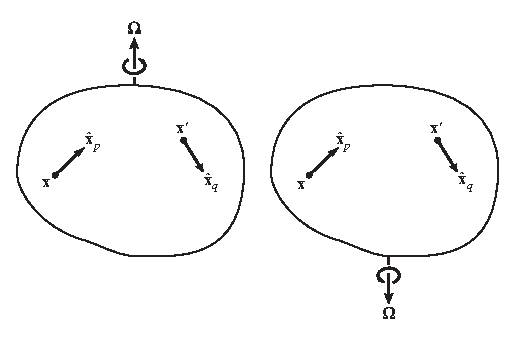
\includegraphics{../figures/chap04/fig03.eps}
\end{center}
\caption[seisrotrep]{\label{fig4.3}
自转地球上的地震互易性:作用在地球上~${\bf x}^{\prime}$~处~$\hat{\bf x}_q$~方向点力所造成的在$\bf x$~处响应的~$\hat{\bf x}_p$~分量({\em 左图})等于作用在逆转地球上~$\bf x$处~$\hat{\bf x}_p$~方向点力所造成的在~${\bf x}^{\prime}$~处响应的~$\hat{\bf x}_q$~分量({\em 右图})。格林张量和逆转格林张量的分量之间的关系:~$G_{pq}({\bf x},{\bf x}^{\prime};t)
=\overline{G}_{qp}({\bf x}^{\prime},{\bf x};t)$。
\index{force!point}%
\index{point force}%
}
\end{figure}

在取~(\ref{4.rotck3})~与~$\bz_{k'}$~和~$\bz_{k'}^*$~的六维内积之前,必须先将平凡模式从本征解中剔除;因此,公式~(\ref{4.rotGreensum})~中的求和是针对所有本征频率为正~($\omega_k>0$)~的非平凡模式。严格来说,倾斜模式不是平凡模式,因此它应该被包括在内;然而,由于地震这样的内部源对地球没有净力矩的作用,所以不能激发倾斜模式。我们把从叠加中剔除了倾斜模式和所有平凡模式的~$\bG$~称为{\em 地震格林张量\/}。
\index{Green tensor!seismic}%
\index{seismic Green tensor}%
\textcite{wahr81a}~第一个利用上述方法得到了自转地球上的格林张量;\textcite{dahlen&smith75}~和~Dahlen (\citeyear{dahlen77};
\citeyear{dahlen78}; \citeyear{dahlen80})~给出了在优雅程度上稍显逊色的三维推导。值得注意的是,即使存在本征频率的偶然简并,~(\ref{4.rotGreensum})~式也是适用的;
\index{degeneracy!accidental}%
\index{accidental degeneracy}%
对于我们将在第~6.2.3~节和第~6.3.3~节中推导的非弹性地球的模式叠加格林张量,情况却并非如此。倾斜模式虽然在地震学应用中可以忽略,但它对由于外部日月潮汐力矩所引起的地球章动响应却有显著影响;
\index{tilt-over mode}%
\index{mode!tilt-over}%
\index{free core nutation}%
还有一个相邻的非刚体模式,称为自由核章动或近周日自由摆动,在这方面起着更为重要的作用~(Smith \citeyear{smith77}; Wahr \citeyear{wahr81c})。
\index{nearly diurnal free wobble}%
\index{Green tensor!rotating Earth|)}%
\index{tensor!Green!rotating|)}%

\renewcommand{\thesubsection}{$\!\!\!\raise1.3ex\hbox{$\star$}\!\!$
\arabic{chapter}.\arabic{section}.\arabic{subsection}}
%\subsection{Response to a transient force}
\subsection{对短时力的响应}
\index{transient force!rotating Earth|(}%
\index{force!transient|(}%
\label{4.sec.rottrans}
\renewcommand{\thesubsection}{\arabic{chapter}.\arabic{section}.\arabic{subsection}}

在体力密度~$\bef$~和面力密度~$\bt$~作用下的完整响应为
\eqa
\label{4.Rotconv}
\lefteqn{
\bs(\bx,t)=\int_{-\infty}^t\int_{\subearth}\bG(\bx,\bx';t-t')\cdot\bef(\bx',t')
\,dV'\,dt'} \nonumber \\
& & \mbox{}\qquad\qquad+\int_{-\infty}^t\int_{\partial\subearth}\bG(\bx,\bx';t-t')
\cdot\bt(\bx',t')\,d\/\Sigma'\,dt' \nonumber \\
&&\mbox{}\qquad\qquad\qquad\qquad\qquad+\bs_{\rm triv}(\bx,t),
\ena
其中~$\bs_{\rm triv}$~是平凡模式的线性组合,是仍待确定的。暂且忽略它微不足道的贡献,将格林张量~(\ref{4.rotGreensum})~代入~(\ref{4.Rotconv})~式,我们得到以模式叠加表示的地震响应:
\eq
\label{4.rotsxt1}
\bs(\bx,t)=\Re{\rm e}\sum_{k}(i\omega_k)^{-1}\bs_k(\bx)\int_{-\infty}
^tC_k(t')\exp i\omega_k(t-t')\,dt',
\en
其中
\eq
\label{4.rotAkt1}
C_k(t)=\int_{\subearth}\bef(\bx,t)\cdot\bs_k^*(\bx)\,dV+
\int_{\spar\subearth}\bt(\bx,t)\cdot\bs_k^*(\bx)\,d\/\Sigma.
\en
类似于~(\ref{4.nrsxt2}),我们对时间做分部积分,可以得到等价的结果:
\eqa
\label{4.rotsxt2}
\lefteqn{
\bs(\bx,t)=\Re{\rm e}\sum_{k}\omega_k^{-2}\bs_k(\bx)\int_{-\infty}^t\p_{t'}
C_k(t')[1-\exp i\omega_k(t-t')]\,dt',} \nonumber \\
&&\mbox{}
\ena
其中
\eq
\label{4.rotAkt2}
\p_tC_k(t)=\int_{\subearth}\p_t\bef(\bx,t)\cdot\bs_k^*(\bx)\,dV+
\int_{\spar\subearth}\p_t\bt(\bx,t)\cdot\bs_k^*(\bx)\,d\/\Sigma.
\en

与无自转地球一样,我们更感兴趣的是等同于地震的{\em 短时力\/}的响应,
\index{force!transient}%
\index{transient force}%
该短时力在某一起始时刻~$t_0$~之前为零,在~$t_{\rm f}$~时刻之后达到恒定值~$\bef_{\rm f}$~和~$\bt_{\rm f}$。在破裂停止之后,这种力所产生的位移为
%%%
\eq
\label{4.rotsxt3}
\bs(\bx,t)=\Re{\rm e}\sum_k\omega_k^{-2}[c_k^{\rm f}-c_k\exp(i\omega_kt)]
\bs_k(\bx),\quad t\geq t_{\rm f},
\en
其中
\eq
\label{4.rotstat}
c_k^{\rm f}=\int_{\subearth}\bef_{\rm f}(\bx)\cdot\bs_k^*(\bx)\,dV+
\int_{\spar\subearth}\bt_{\rm f}(\bx)\cdot\bs_k^*(\bx)\,d\/\Sigma,
\en
\eqa
\lefteqn{
c_k=\int_{t_0}^{t_{\rm f}}\int_{\subearth}\p_t\bef(\bx,t)
\cdot\bs_k^*(\bx)\exp(-i\omega_kt)\,dV\,dt}
\nonumber \\
&&\mbox{}+
\int_{t_0}^{t_{\rm f}}\int_{\spar\subearth}\p_t\bt(\bx,t)
\cdot\bs_k^*(\bx)\exp(-i\omega_kt)\,d\/\Sigma\,dt.
\ena
由于地球的非弹性,公式~(\ref{4.rotsxt3})~中的{\em 自由振荡\/}项~$c_k\exp(i\omega_kt)$~随时间衰减;
\index{free oscillations}%
在长时间极限~$t\rightarrow \infty$~下,最终的{\em 静态位移\/}为
\index{static displacement}%
\index{displacement!static}%
\index{response!static}%
\eq
\label{4.rotsstat}
\bs_{\rm f}(\bx)=\Re{\rm e}
\sum_k\omega_k^{-2}c_k^{\rm f}\bs_k(\bx),
\en
而破裂停止后的质点{\em 加速度\/}则为
\index{acceleration}%
\index{particle acceleration}%
\eq
\label{4.rotaxt}
\ba(\bx,t)=\Re{\rm e}\sum_kc_k\exp (i\omega_kt)
_{\,}\bs_k(\bx),\quad t\geq t_{\rm f}.
\en
令~$c_k=a_k-ib_k$,$c_k^{\rm f}=a_k^{\rm f}-ib_k^{\rm f}$,公式~(\ref{4.rotsxt3})--(\ref{4.rotaxt})~成为~(\ref{4.nrsxt3})--(\ref{4.nraxt})。(\ref{4.rotaxt})~式的叠加是在~$t\geq t_{\rm f}$~时能够被地震仪记录到的运动的完备的表述;我们接下来将注意力转向~(\ref{4.Rotconv})~式中的平凡模式响应~$\bs_{\rm triv}$。
\index{transient force!rotating Earth|)}%
\index{force!transient|)}%

\renewcommand{\thesubsection}{$\!\!\!\raise1.3ex\hbox{$\star$}\!\!$
\arabic{chapter}.\arabic{section}.\arabic{subsection}}
%\subsection{Change in rotation rate}
\subsection{自转速率的变化}
\index{rotation!change in|(}%
\renewcommand{\thesubsection}{\arabic{chapter}.\arabic{section}.\arabic{subsection}}

只有一个平凡模式---轴向转动模式---可以被地壳或地幔中的地震所激发;
\index{axial spin mode}%
\index{mode!axial spin}%
\index{mode!trivial}%
\index{trivial mode}%
地转模式因为都局限于地球的液态区域是不能被激发的,而平动模式只能被对地球有净力作用的源激发。轴向转动模式即使在对地球净力矩为零时也能被激发,原因是静态形变~$\bs_{\rm f}$~会导致主转动惯量~$C$~的扰动,
\index{moment of inertia!principal}%
必须通过自转速率~$\Omega$~的变化来抵消。\textcite{wahr81a}确定了一个随时间变化的任意力密度~$\bef$、$\bt$~所引起的无穷小转动响应。我们在此直接引用他的结果:
\eq
\bs_{\rm triv}(\bx,t)=c_{\rm triv}(t)(\bzh\times\bx),
\en
其中
\eqa
\label{4.wahr}
\lefteqn{
c_{\rm triv}(t)=2(C\Omega)^{-1}\Re{\rm e}\sum_k\omega_k^{-2}\int_
{\subearth}\rho^0\bs_k\cdot\bdel\psi\,dV} \nonumber \\
&&\mbox{}\qquad\qquad\times\int_{-\infty}^tC_k(t')\,dt'.
\ena
对于短时力,~(\ref{4.wahr})~式中的时间依赖性简化为
\eq
\label{4.wahr2}
\int_{-\infty}^tC_k(t')\,dt'=\int_{t_{\rm 0}}^{t_{\rm f}}C_k(t')\,dt'
+c_k^{\rm f}(t-t_{\rm f}).
\en
(\ref{4.wahr})~是在位移~$\bs_{\rm triv}$~可被线性化的假设下推导出来的, 而且~(\ref{4.wahr2})~很显然只在~$t_{\rm f}$~之后的短时间内成立。然而,上式中正比于~$t-t_{\rm f}$~的项可以被解释为{\em 
地球自转速率无穷小的变化\/}:
\index{rotation!change in}%
\eq
\label{4.deltaOm}
\delta\Omega=2(C\Omega)^{-1}\Re{\rm e}\sum_k\omega_k^{-2}c_k^{\rm f}
\int_{\subearth}\rho^0\bs_k\cdot\bdel\psi\,dV.
\en
地震位移~(\ref{4.rotsxt3})~式可以被视为在以新的角速度~$\Omega+\delta\Omega$~转动的参照系中的观察者所测量的位移。这同将~$\bs_{\rm f}$~解释为代表了地球的无穷小静态形变是一致的。

(\ref{4.deltaOm})~式也可用第一性原理推导出来,根据角动量守恒定律,自转速率的变化~$\delta\Omega$~与主转动惯量的无穷小变化~$\delta C$~之间有关系
\eq
\label{4.angmom}
C\hspace{1.0 mm}\delta\Omega+\delta C\hspace{1.0 mm}\Omega=0.
\en
与质量的静态重新分布相关的转动惯性张量~$\bC=\int_{\subearth}\rho^0[(\bx\cdot\bx)\bI-\bx\bx]\,dV$~的一阶扰动为
\index{inertia tensor}%
\index{tensor!inertia}%
\eq
\bdelta\bC=\int_{\subearth}\rho^0[2(\bx\cdot\bs_{\rm f})\bI-\bx\bs_{\rm f}
-\bs_{\rm f}\bx]\,dV.
\en
令~$\delta C=\bzh\cdot\bdelta\bC\cdot\bzh$,将其代入~(\ref{4.angmom}),我们得到
\eq
\delta\Omega=2(C\Omega)^{-1}\int_{\subearth}\rho^0\bs_{\rm f}
\cdot\bdel\psi\,dV,
\en
上式与~(\ref{4.deltaOm})~一致。
\index{rotation!change in|)}%
\index{normal mode!rotating Earth|)}%

%\section{Hydrostatic Earth Model}
\section{流体静力学地球模型}
\index{normal mode!hydrostatic Earth|(}%

本章中得到的所有结果只需很小的改动都适用于具有流体静力学初始应力的地球模型。我们在此对必要的修改做一个扼要的介绍,为了简明起见,将注意力局限在无自转情况;通过类比可以很容易地得到自转流体静力学地球的相应结果。

无自转流体静力学地球的本征频率~$\omega$~和本征函数~$\bs$~来自于求解方程:
\eqa
\label{4.nrhydromom}
\lefteqn{
-\omega^2\rho^0\bs-\bdel\cdot\bT^{\rm L1}}
\nonumber \\
&&\mbox{}+\bdel(\rho^0\bs\cdot\bdel\phi^0)
+\rho^0\bdel\phi^{\rm E1}+\rho^{\rm E1}\bdel\phi^0=\bzero,
\ena
以及边界条件
\eq
\label{4.hydrobc1}
\bnh\cdot\bT^{\rm L1}=\bzero\quad\mbox{在 $\p\earth$上},
\en
\eq
\label{4.hydrobc2}
[\bnh\cdot\bT^{\rm L1}]^+_-=\bzero\quad\mbox{在 $\Sigma_{\rm SS}$上},
\en
\eq
\label{4.hydrobc3}
[\bnh\cdot\bT^{\rm L1}]^+_-
=\bnh[\bnh\cdot\bT^{\rm L1}\cdot\bnh]^+_-=\bzero
\quad\mbox{在 $\Sigma_{\rm FS}$上}.
\en
拉格朗日-柯西应力增量~$\bT^{\rm L1}$~和欧拉密度微扰~$\rho^{\rm E1}$~分别由~$\bT^{\rm L1}=\bGamma\!:\!\beps$和$\rho^{\rm E1}=-\bdel\cdot(\rho^0\bs)$~给定。
\index{stress!Cauchy}%
\index{Cauchy stress}%

%\subsection{Hermiticity and orthonormality}
\subsection{厄米特性与正交归一性}
\index{orthonormality!hydrostatic Earth|(}%
\label{4.sec.hyHerm}

我们可以将简正模式的本征值问题~(\ref{4.nrhydromom})--(\ref{4.hydrobc3})~写为符号形式
\eq
\sH\bs=\omega^2\bs,
\en
其中
\eq
\label{4.Hhydro}
\rho^0\sH\bs=-\bdel\cdot\bT^{\rm L1}
+\bdel(\rho^0\bs\cdot\bdel\phi^0)
+\rho^0\bdel\phi^{\rm E1}+\rho^{\rm E1}\bdel\phi^0.
\en
利用高斯定理及边界条件~(\ref{4.hydrobc1})--(\ref{4.hydrobc2})~可得:
\eqa
\label{4.HYHERM1}
\lefteqn{\langle\bs,\sH\bs'\rangle
=\int_{\subearth}
[\beps\!:\!\bGamma\!:\!\beps'
+\rho^0\bs\cdot\bdel\phi^{{\rm E1}\prime}
+\rho^0\bs\cdot\bdel\bdel\phi^0\cdot\bs'} \nonumber \\
&&\mbox{}\qquad\qquad\qquad\qquad+\rho^0\bdel\phi^0\cdot(\bs\cdot\bdel\bs'
-\bs\bdel\cdot\bs')]\,dV,
\ena
\eqa
\label{4.HYHERM2}
\lefteqn{\langle\bs',\sH\bs\rangle
=\int_{\subearth}
[\beps'\!:\!\bGamma\!:\!\beps
+\rho^0\bs'\cdot\bdel\phi^{\rm E1}
+\rho^0\bs'\cdot\bdel\bdel\phi^0\cdot\bs} \nonumber \\
&&\mbox{}\qquad\qquad\qquad\qquad+\rho^0\bdel\phi^0\cdot(\bs'\cdot\bdel\bs
-\bs'\bdel\cdot\bs)]\,dV.
\ena
利用麦克斯韦关系~$\Gamma_{ijkl}=\Gamma_{klij}$、引力对称性~(\ref{4.gravid})~以及等式
\eqa
\label{4.GRAVID}
\lefteqn{\int_{\subearth}
\rho^0\bdel\phi^0\cdot(\bs\cdot\bdel\bs'
-\bs\bdel\cdot\bs')]\,dV} \nonumber \\
&&\mbox{}\qquad=\int_{\subearth}
\rho^0\bdel\phi^0\cdot(\bs'\cdot\bdel\bs
-\bs'\bdel\cdot\bs)]\,dV,
\ena
可以看到~(\ref{4.HYHERM1})~和~(\ref{4.HYHERM2})~两式是相等的。
因此,算子~$\sH$~相对于~(\ref{4.inprod})~定义的内积是具厄米特性质的:
\eq
\label{4.HYHERM}
\langle\bs,\sH\bs'\rangle=\langle\sH\bs,\bs'\rangle
=\langle\bs',\sH\bs\rangle.
\en
\index{Hermitian operator}%
\index{operator!Hermitian}%
\index{self-adjoint operator}%
\index{operator!self-adjoint}%
在得到~(\ref{4.GRAVID})~式的过程中,我们在~$\earth$~内和~$\Sigma$~上分别应用了体积和表面的流体静力学条件~$\bdel\rho^0\times\bdel\phi^0=\bzero$~和~$\bdel^{\Sigma}\phi^0=\bzero$。厄米特对称性~(\ref{4.HYHERM})~确保了简正模式的正交关系~(\ref{4.NORMAL})~能够适用于无自转流体静力学地球模型;我们仍然利用~$\langle\bs,\bs\rangle=1$~来对本征函数做归一化。
\index{orthonormality!hydrostatic Earth|)}%

%\subsection{Rayleigh's principle}
\subsection{瑞利原理}
\index{Rayleigh's principle!hydrostatic Earth|(}%

势能泛函~(\ref{4.Vdef})~和修改后的势能泛函~(\ref{4.Vdef2})~成为
\index{functional!potential energy}%
\index{potential energy functional}%
\eqa
\label{4.Vhydrodef}
\lefteqn{\sV=\int_{\subearth}
[\beps\!:\!\bGamma\!:\!\beps
+\rho^0\bs\cdot\bdel\phi^{\rm E1}+\rho^0
\bs\cdot\bdel\bdel\phi^0\cdot\bs} \nonumber \\
&&\mbox{}\qquad\qquad\qquad\qquad+\rho^0\bdel\phi^0\cdot(\bs\cdot\bdel\bs
-\bs\bdel\cdot\bs)]\,dV,
\ena
\eqa
\label{4.Vhydrodef2}
\lefteqn{\sV'=\int_{\subspace}
[\beps\!:\!\bGamma\!:\!\beps
+2\rho^0\bs\cdot\bdel\phi^{\rm E1}+\rho^0
\bs\cdot\bdel\bdel\phi^0\cdot\bs} \\
&&\mbox{}+\rho^0\bdel\phi^0\cdot(\bs\cdot\bdel\bs
-\bs\bdel\cdot\bs)+(4\pi G)^{-1}
\bdel\phi^{\rm E1}\cdot\bdel\phi^{\rm E1}]\,dV. \nonumber
\ena
利用这两个泛函做替换,各种形式的瑞利原理仍然成立。当且仅当~$\omega$~和~$\bs$~满足频率域动量方程和边界条件~(\ref{4.nrhydromom})--(\ref{4.hydrobc3})~时,对于任意可容许变化~$\bdelta\bs$,作用量~$\sI=\half(\omega^2\sT-\sV)$~是稳定的,
\index{action}%
同样地,当且仅当~$\bs$~和~$\phi^{\rm E1}$~满足势函数边值问题~(\ref{4.divgam})~时,对于任意的独立可容许变化~$\bdelta\bs$~和~$\delta\phi^{\rm E1}$,修改后的作用量~$\sI'=\half(\omega^2\sT-\sV')$~是稳定的。
\index{action!modified}%
\index{modified action}%
根据等式~(\ref{3.twoints}),不带撇号与带撇号的势能泛函和作用量是相等的。对于所有本征解~$\bs$、$\phi^{\rm E1}$,两种流体静力学作用量的稳定值都是~$\sI=\sI'=0$。
\index{Rayleigh's principle!hydrostatic Earth|)}%

%\subsection{Lagrangian and energy density}
\subsection{拉格朗日量与能量密度}
\index{Lagrangian density|(}%
\index{energy density|(}%

无自转流体静力学地球的作用量可以写为:
\index{action}%
\index{action!modified}%
\index{modified action}%
\eq
\label{4.hydroact}
\sI=\int_{\subearth}L(\bs,\bdel\bs)\,dV,\qquad
\en
\eq
\label{4.hydroact2}
\sI'=\int_{\subspace}L'(\bs,\bdel\bs,\bdel\phi^{\rm E1})\,dV,
\en
其中
\eqa
\label{4.ZOOTME}
\lefteqn{L=\half[\omega^2\rho^0\bs\cdot\bs
-\beps\!:\!\bGamma\!:\!\beps
-\rho^0\bs\cdot\bdel\phi^{\rm E1}} \nonumber \\
&&\mbox{}\qquad-\rho^0
\bs\cdot\bdel\bdel\phi^0\cdot\bs
-\rho^0\bdel\phi^0\cdot(\bs\cdot\bdel\bs
-\bs\bdel\cdot\bs)],
\ena
\eqa
\label{4.ZOOT}
\lefteqn{L'=\half[\omega^2\rho^0\bs\cdot\bs
-\beps\!:\!\bGamma\!:\!\beps
-2\rho^0\bs\cdot\bdel\phi^{\rm E1}} \nonumber \\
&&\mbox{}\qquad-\rho^0
\bs\cdot\bdel\bdel\phi^0\cdot\bs
-\rho^0\bdel\phi^0\cdot(\bs\cdot\bdel\bs
-\bs\bdel\cdot\bs) \nonumber \\
&&\mbox{}\qquad\qquad\qquad-(4\pi G)^{-1}
\bdel\phi^{\rm E1}\cdot\bdel\phi^{\rm E1}].
\ena
相应的频率域能量密度~$E=\omega\p_{\omega}L-L$~和~$E'=\omega\p_{\omega}L'-L'$~为
\eqa
\lefteqn{E=\half[\omega^2\rho^0\bs\cdot\bs
+\beps\!:\!\bGamma\!:\!\beps
+\rho^0\bs\cdot\bdel\phi^{\rm E1}} \nonumber \\
&&\mbox{}\qquad+\rho^0
\bs\cdot\bdel\bdel\phi^0\cdot\bs
+\rho^0\bdel\phi^0\cdot(\bs\cdot\bdel\bs
-\bs\bdel\cdot\bs)],
\ena
\eqa
\lefteqn{E'=\half[\omega^2\rho^0\bs\cdot\bs
+\beps\!:\!\bGamma\!:\!\beps
+2\rho^0\bs\cdot\bdel\phi^{\rm E1}} \nonumber \\
&&\mbox{}\qquad+\rho^0
\bs\cdot\bdel\bdel\phi^0\cdot\bs
+\rho^0\bdel\phi^0\cdot(\bs\cdot\bdel\bs
-\bs\bdel\cdot\bs) \nonumber \\
&&\mbox{}\qquad\qquad\qquad+(4\pi G)^{-1}
\bdel\phi^{\rm E1}\cdot\bdel\phi^{\rm E1}].
\ena
能量密度的体积分~$\sE=\half(\omega^2\sT+\sV)
=\half(\omega^2\sT+\sV')$~是以~$\bs(\bx)\cos\omega t$~或~$\bs(\bx)\sin\omega t$~做自由振荡的一个周期中,地球平均动能与势能之和的四倍。
\index{Lagrangian density|)}%
\index{energy density|)}%

%\subsection{Elastic and gravitational energy}
\subsection{弹性能与引力能}
\index{energy!elastic|(}
\index{elastic energy|(}
\index{energy!gravitational|(}
\index{gravitational energy|(}
\label{4.sec.hyenergy}

与时间域中一样,我们可以将无自转流体静力学地球的一个模式的势能分为独立的弹性能和引力能:
\eq
\label{4.PART1}
\sV=\sV_{\rm e}+\sV_{\rm g},
\en
其中
\eq
\label{4.Velasdef}
\sV_{\rm e}=\int_{\subearth}
(\beps\!:\!\bGamma\!:\!\beps)\,dV,
\en
\eqa
\label{4.Vgravdef}
\lefteqn{\sV_{\rm g}=\int_{\subearth}[
\rho^0\bs\cdot\bdel\phi^{\rm E1}+\rho^0
\bs\cdot\bdel\bdel\phi^0\cdot\bs} \nonumber \\
&&\mbox{}\qquad\qquad\qquad+\rho^0\bdel\phi^0\cdot(\bs\cdot\bdel\bs
-\bs\bdel\cdot\bs)]\,dV.
\ena
在归一化条件~$\sT=1$~下,能量均分关系~$\omega^2\sT=\sV$~成为
\eq
f_{\rm e}+f_{\rm g}=1,
\en
其中~$f_{\rm e}=\omega^{-2}\sV_{\rm e}$~和~$f_{\rm g}=\omega^{-2}\sV_{\rm g}$~为{\em 弹性能占比\/}和{\em 引力能占比}。
\index{energy!fractional}%
\index{fractional energy}%
非平凡模式的弹性能必定是非负的,即~$\sV_{\rm e}\geq 0$,而引力能则可正可负,取决于引力的作用是保持还是破坏稳定。
\index{energy!elastic|)}
\index{elastic energy|)}
\index{energy!gravitational|)}
\index{gravitational energy|)}

%\subsection{Non-gravitating limit}
\subsection{无引力的极限情形}
\index{non-gravitating limit|(}%
\index{body-wave limit|(}%

从物理上讲,我们预期长程的引力恢复力对短周期、短波长振荡的影响是可以忽略不计的。
\index{force!long-range}%
\index{long-range force}%
为了确定一个忽略引力的标准,我们对比一下~(\ref{4.nrhydromom})~中各项的相对大小:
\begin{displaymath}
\begin{array}{l}
\mbox{惯性项:}\;\;-\omega^2\rho^0\bs, \\
\mbox{弹性项:}\;\;-\bdel\cdot\bT^{\rm L1}, \\
\mbox{引力项:} \;\;\;\bdel(\rho^0\bs\cdot\bdel\phi^0)
+\rho^0\bdel\phi^{\rm E1}+\rho^{\rm E1}\bdel\phi^0.
\end{array}
\end{displaymath}
利用~$\rho^{\rm E1}=-\bdel\cdot(\rho^0\bs)$~和~$\del^2\phi^{\rm E1}=4\pi G\rho^{\rm E1}$~来估计密度增量和引力势函数增量的大小,我们发现
\eq \label{4.compare2}
\|\hspace{-0.4 mm}-\omega^2\rho^0\bs\|\approx
\|\hspace{-0.4 mm}-\bdel\cdot\bT^{\rm L1}\|\approx\om^2(\rho^0S),
\en
\eq \label{4.compare3}
\|\bdel(\rho^0\bs\cdot\bdel\phi^0)+\rho^0\bdel\phi^{\rm E1}
+\rho^{\rm E1}\bdel\phi^0\|\approx 4\pi G\rho^0(\rho^0S),
\en
其中~$S\approx\|\bs\|$~为质点位移的大小。比较~(\ref{4.compare2})~和~(\ref{4.compare3}),我们看到,只有在振荡的频率低到
\eq \label{4.needlastmin}
\om\approx(4\pi G\rho^0)^{1/2}
\en
时,引力的影响才会与惯性和弹性的影响相当。假设地球的平均密度为~$\rho^0\approx5500\,\mbox{kg/m}^3$,我们发现对应的周期为~$2\pi/\omega\approx3000$~秒。无独有偶,这一数值几乎与受引力剧烈影响的橄榄球模式~${}_0{\rm S}_{2}$~的周期相等(见第~1.1~节和第~8.8.10~节)。实践上,在周期短于大约~30~秒的体波、区域波和勘探地震学中,引力是被忽略的。

在无引力的近似下,波的传播满足经典的弹性动力学方程
\eq \label{4.classeqmom}
-\omega^2\rho^0\bs-\bdel\cdot\bT^{\rm L1}=\bzero\quad
\mbox{其中}\quad\bT^{\rm L1}=\bGamma\!:\!\beps.
\en
对应于~(\ref{4.classeqmom})~的经典拉格朗日量和能量密度为
\eq \label{4.classLE}
L=\half(\om^2\rho^0\bs\cdot\bs-\beps\!:\!\bGamma\!:\!\beps),\qquad
E=\half(\om^2\rho^0\bs\cdot\bs+\beps\!:\!\bGamma\!:\!\beps).
\en
在这种近似下,振荡的势能当然是纯弹性的;由于~$\sV=\sV_{\rm e}\geq 0$,无引力的液态或固态弹性体具有{\em 内在稳定性\/}。
\index{stability}%

也可以忽略引力势函数的一阶微扰~$\phi^{\rm E1}$,但保留初始势函数~$\phi^0$。这样,(\ref{4.nrhydromom})~退化为一个纯微分本征值问题:
\eq \label{4.Cowling}
-\omega^2\rho^0\bs-\bdel\cdot\bT^{\rm L1}
+\bdel(\rho^0\bs\cdot\bdel\phi^0)
+\rho^{\rm E1}\bdel\phi^0=\bzero.
\en
在天体物理学中,方程~(\ref{4.Cowling})~的声波形式,其中~$\bT^{\rm L1}=-\kappa(\bdel\cdot\bs)\bI$,被称作~{\em Cowling~近似\/};
\index{Cowling approximation}%
它使得在探究太阳和其它恒星的受引力主导的振荡~($f_{\rm g}\gg f_{\rm e}$)~和受声波主导的振荡~($f_{\rm e}\gg f_{\rm g}$)~的定性特征时,
\index{Sun}%
\index{star}%
不需要去求解一个积分-微分方程~(Cowling \citeyear{cowling41}; Cox \citeyear{cox80}; Unno, Osaki, Ando, Saio \& Shibahashi \citeyear{unno&al89})。所有观测到的地球的振荡都是以弹性特征为主的;因此,Cowling~近似在类地地震学上几乎没有得到任何应用。
\index{non-gravitating limit|)}%
\index{body-wave limit|)}%

\renewcommand{\thesection}{$\!\!\!\raise1.3ex\hbox{$\star$}\!\!$
\arabic{chapter}.\arabic{section}}
%\section{Response of an Idealized Seismometer}
\section{理想地震仪的响应}
\index{response!seismometer|(}%
\index{seismometer!response of|(}%
\index{seismometer response|(}%
\label{4.sec.accel}
\renewcommand{\thesection}{\arabic{chapter}.\arabic{section}}

在将~(\ref{4.nraxt})~和~(\ref{4.rotaxt})~这种以模式叠加表示的加速度响应~$\ba(\bx,t)$~应用于分析地震数据之前,我们还必须考虑记录仪器的响应。遵循~\textcite{gilbert80}~和~\textcite{wahr81b},我们将三分量地震仪模拟为一个在固定于质点~$\bx$~上的外壳内的有三个自由度的传感器或质量。在下面的讨论中,我们会考虑地球自转~$\bOmega$~对地震仪的影响,因为它并不带来任何额外的大麻烦。

令~$\bnu$~表示地震仪质量相对于仪器外壳的位移;其相对于均匀转动参照系的位置则为~$\br=\bx+\bs+\bnu$。传感器的运动方程为
\eq
\label{4.seismo1}
\p_t^2\br+2\bOmega\times\p_t\br+\bOmega\times(\bOmega\times\br)
=\bF+\bg^{\rm L},
\en
其中~$\bg^{\rm L}$~为地球对质点~$\bx$~的总的引力作用,$\bF$~为仪器所产生的机电恢复力。
\index{force!feedback}%
\index{feedback force}%
将依赖于相对位移~$\bnu$~的项移到左边,所有其它项移到右边,方程~(\ref{4.seismo1})~成为
\eqa
\label{4.seismo2}
\lefteqn{
\p_t^2\bnu+2\bOmega\times\p_t\bnu+\bOmega\times(\bOmega\times\bnu)
=\bF-\bdel(\phi^0+\psi)} \nonumber \\
&&\mbox{}-\p_t^2\bs-2\bOmega\times\p_t\bs
-\bdel\phi^{\rm E1}-\bs\cdot\bdel\bdel(\phi^0+\psi),
\ena
这里我们使用了一阶关系~(\ref{3.gL1phiL1})~以及离心势函数等式~$\bOmega\times(\bOmega\times\bx)=\bdel\psi$~和~$\bOmega\times(\bOmega\times\bs)=\bs\cdot\bdel\bdel\psi$。现代的力平衡式地震仪是通过对恢复力~$\bF$~的持续调整,使得传感器相对于仪器外壳的位置保持不变;
\index{force-balance seismometer}%
\index{seismometer!force-balance}%
在没有任何地面运动时,平衡力为~$\bF^0=\bdel(\phi^0+\psi)$,而要保持~$\bnu=\bzero$~所需的反馈力则为~$\bF=\bdel(\phi^0+\psi)+\p_t^2\bs+2\bOmega\times\p_t\bs
+\bdel\phi^{\rm E1}+\bs\cdot\bdel\bdel(\phi^0+\psi)$。
所记录到的信号正比于
\eqa
\label{4.seismo3}
\lefteqn{
A=\bnuh\cdot\bF-\bnuh^0\cdot\bF^0=
(\bnuh-\bnuh^0)\cdot\bdel(\phi^0+\psi)} \nonumber \\
&&\mbox{}+\bnuh^0\cdot[\p_t^2\bs+
2\bOmega\times\p_t\bs+\bdel\phi^{\rm E1}+\bs\cdot\bdel\bdel(\phi^0+\psi)],
\ena
其中~$\bnuh$~和~$\bnuh^0$~分别为仪器的瞬时和平衡偏振方向。在得到第二个等式时, 我们忽略了~$\bs$~的二阶项。

对于{\em 垂直地震仪\/},
\index{seismometer!vertical}%
有$\bnuh^0=-\hat{\bgamma}^0$~和~$\bnuh-\bnuh^0=-\bdel_{\!\perp}\bs\cdot\bnuh^0$,其中~$\bgamma^0=-\bdel(\phi^0+\psi)$~为扰动前的引力与向心加速度之和,$\bdel_{\!\perp}=\bdel-\hat{\bgamma}^0(\hat{\bgamma}^0\cdot\bdel)$~为垂直于偏振方向的梯度。将这些关系代入~(\ref{4.seismo3})~式,并利用正交性~$\hat{\bgamma}^0\cdot\bdel_{\!\perp}=0$~和微分对称性~$(\bdel_{\!\perp}\bnuh^0)^{\rm T}=\bdel_{\!\perp}\bnuh^0$,我们得到
\eq \label{4.seismovert}
A_{\rm vert}=\bnuh^0\cdot(\p_t^2\bs+2\bOmega\times\p_t\bs
+\bdel\phi^{\rm E1})+\bs\cdot\bdel\gamma^0,
\en
其中~$\gamma^0=\|\bgamma^0\|$。从~(\ref{4.seismovert})~我们看到,垂直偏振的仪器除了对质点加速度~$\p_t^2\bs$~的响应之外,还有对科里奥利加速度~$2\bOmega\times\p_t\bs$、引力势函数微扰~$\bdel\phi^{\rm E1}$~以及自由空气重力变化~$\bs\cdot\bdel\gamma^0$~的响应。对于{\em 水平地震仪\/},
\index{seismometer!horizontal}%
则有~$\bnuh^0\cdot\hat{\bgamma}^0=0$~和~$\bnuh-\bnuh^0=\bnuh^0\cdot\bdel\bs$;
此时~(\ref{4.seismo3})~成为
\eq
A_{\rm horiz}=\bnuh^0\cdot[\p_t^2\bs+2\bOmega\times\p_t\bs
+\bdel\phi^{\rm E1}-\bdel(\bgamma^0\cdot\bs)].
\en
这样的仪器除了对质点加速度~$\p_t^2\bs$~的响应之外,还有对科里奥利加速度~$2\bOmega\times\p_t\bs$、引力势函数微扰~$\bdel\phi^{\rm E1}$~以及地面倾斜~$\bdel(\bgamma^0\cdot\bs)$~的响应。

总之,垂直或水平偏振的加速度仪所感受到的并不是简单的仪器外壳加速度~$\ba=\p_t^2\bs$,
\index{accelerometer}%
而是{\em 修改后的加速度\/}
\index{acceleration!modified}%
\index{modified acceleration}%
\eqa
\lefteqn{\bA=\p_t^2\bs+2\bOmega\times\p_t\bs
+\bdel\phi^{\rm E1}-\bnuh^0\bs\cdot\bdel(\bnuh^0\cdot\bgamma^0)} \nonumber \\
&&\mbox{}-\bnuh^0[\bnuh^0-\hat{\bgamma}^0(\bnuh^0\cdot\hat{\bgamma}^0)]
\cdot\bdel(\bgamma^0\cdot\bs),
\ena
其中~$\bnuh^0$~为所观测的分量。在无自转的地球上,我们可以通过对~(\ref{4.nraxt})~式中的本征函数~$\bs_k(\bx)$~做下面的替换来引入这些自引力效应:
\eqa
\label{4.seismo6}
\lefteqn{\bs_k\rightarrow\bs_k-\omega_k^{-2}\{\bdel\phi^{\rm E1}_k
-\bnuh^0\bs_k\cdot\bdel(\bnuh^0\cdot\bg^0)} \nonumber \\
&&\mbox{}-\bnuh^0[\bnuh^0-\hat{\bg}^0(\bnuh^0\cdot\hat{\bg}^0)]
\cdot\bdel(\bg^0\cdot\bs_k)\}.
\ena
在自转地球上,我们还必须考虑科里奥利力和离心力的影响,
\index{centrifugal force}%
\index{force!centrifugal}%
此时我们需要在~(\ref{4.rotaxt})~中做如下替换:
\eqa
\label{4.seismo7}
\lefteqn{\bs_k\rightarrow\bs_k-2i\omega_k^{-1}\bOmega\times\bs_k
-\omega_k^{-2}\{\bdel\phi^{\rm E1}_k
-\bnuh^0\bs_k\cdot\bdel(\bnuh^0\cdot\bgamma^0)} \nonumber \\
&&\mbox{}-\bnuh^0[\bnuh^0-\hat{\bgamma}^0(\bnuh^0\cdot\hat{\bgamma}^0)]
\cdot\bdel(\bgamma^0\cdot\bs_k)\}.
\ena
我们仍将继续使用简单的公式~(\ref{4.nraxt})~和~(\ref{4.rotaxt})~来表示短时体力和表面力的加速度响应,同时也默认在任何实际应用中,结果应依照~(\ref{4.seismo6})~和~(\ref{4.seismo7})~加以修正。在第~10.4~节中我们会看到,对于一些低频的球型振荡,这些额外的效应是相当重要的。
\index{normal mode!hydrostatic Earth|)}%
\index{seismometer!response of|)}%
\index{seismometer response|)}%
\index{response!seismometer|)}%
